\documentclass[11pt,a4paper]{report}

% Aberstwyth dissertation LaTeX Template
% Authors: Dr. Hannah Dee (hmd1@aber.ac.uk), Neil Taylor (nst@aber.ac.uk)
% This has been adapted from the Leeds Thesis template and the 
% Group Project template for Computer Science in Aberystywth University.
% 
% All comments and suggestions welcome.
%
% Template designed to be used with pdflatex: it may need alteration to
% run with a different LaTeX engine

% To build document on the unix command line, run four commands:
 
% pdflatex dissertation
% bibtex dissertation
% pdflatex dissertation
% pdflatex dissertation

% you will end up with dissertation.pdf 
\usepackage{mmp}

% the following packages are used for citations - You only need to include one. 
%
% Use the cite package if you are using the numeric style (e.g. IEEEannot). 
% Use the natbib package if you are using the author-date style (e.g. authordate2annot). 
% Only use one of these and comment out the other one. 
\usepackage{cite}
%\usepackage{natbib}
\usepackage{graphicx} % Images
\usepackage{tabularx} % Tables
\usepackage[usenames,dvipsnames,svgnames,table]{xcolor}
\usepackage{listings}

\usepackage{color} %red, green, blue, yellow, cyan, magenta, black, white


\definecolor{myBlue}{RGB}{70,130,180} % color values Red, Green, Blue
\definecolor{mylilas}{RGB}{170,55,241}
\definecolor{mygreen}{RGB}{173,255,47}

%\usepackage{hyperref}
\usepackage[colorlinks, urlcolor=myBlue, linkcolor=Black, citecolor=myBlue]{hyperref}
%\usepackage{hypcap}

\lstset{breaklines=true} 

\lstset{numbers=left, numberstyle=\scriptsize\ttfamily, numbersep=10pt, captionpos=b} 
%\lstset{backgroundcolor=\color{Cyan}}
\lstset{basicstyle=\small\ttfamily}
\lstset{framesep=4pt}

\newcommand{\lstjava} {
\lstset{language=Java,%
frame=tb,
    %basicstyle=\color{red}, 
    breaklines=true,%
    morekeywords={matlab2tikz},
    keywordstyle=\color{blue},%
    morekeywords=[2]{1}, keywordstyle=[2]{\color{black}},
    identifierstyle=\color{black},%
    stringstyle=\color{mylilas},
    commentstyle=\color{mygreen},%
    showstringspaces=false,%without this there will be a symbol in the places where there is a space
    numbers=left,%
    numberstyle={\scriptsize\ttfamily},% size of the numbers
    numbersep=10pt, % this defines how far the numbers are from the text
    emph=[1]{for,end,break},emphstyle=[1]\color{Red}, %some words to emphasise
    %emph=[2]{word1,word2}, emphstyle=[2]{style},    
}
}

% Use the following to selectively exclude chapters
%\includeonly{cover,abstract,acknowledge,declare,chapter1,chapter2}
\begin{document}

% all of the include directives below refer to tex files
% so 
\title{Visualising plants and metadata}

% Your name
\author{Si\^{o}n Griffiths}

% Your email 
\authoremail{sig2@aber.ac.uk}

\degreeschemecode{G600} %e.g. G400 
\degreeschemetitle{Software Engineering} % e.g. Computer Science
\degreetype{BEng}

\modulecode{CS39440} % i.e. CS39440, CC39440, CS39620
\moduletitle{Major Project} % i.e. Major Project or Minor Project

\date{18th of April 2016} % i.e. the date of this version of the report

\status{Draft} % Use draft until you create the release version. Then, change this to Release.
\version{1.1}

%The title and name of your supervisor.
\supervisor{Dr. Hannah Dee} 

%The email for your supervisor. 
\supervisoremail{hmd1@aber.ac.uk}

\maketitle



 includes cover.tex - to change the content,
% edit the tex file

\pagenumbering{roman}

% This is the front page

\title{Visualising plants and metadata}

% Your name
\author{Si\^{o}n Griffiths}

% Your email 
\authoremail{sig2@aber.ac.uk}

\degreeschemecode{G600} %e.g. G400 
\degreeschemetitle{Software Engineering} % e.g. Computer Science
\degreetype{BEng}

\modulecode{CS39440} % i.e. CS39440, CC39440, CS39620
\moduletitle{Major Project} % i.e. Major Project or Minor Project

\date{18th of April 2016} % i.e. the date of this version of the report

\status{Draft} % Use draft until you create the release version. Then, change this to Release.
\version{1.1}

%The title and name of your supervisor.
\supervisor{Dr. Hannah Dee} 

%The email for your supervisor. 
\supervisoremail{hmd1@aber.ac.uk}

\maketitle



                        

% Set up page numbering
\pagestyle{empty}

% declarations of originality 
\thispagestyle{empty}

%%%
%%% You must sign the declaration of originality. 
%%%
\begin{center}
    {\LARGE\bf Declaration of originality}
\end{center}

In signing below, I confirm that:

\begin{itemize}
\item{This submission is my own work, except where 
clearly indicated.}

\item{I understand that there are severe penalties for 
Unacceptable Academic Practice, which can lead to loss 
of marks or even the withholding of a degree.}
 
\item{I have read the regulations on Unacceptable Academic 
Practice from the University's Academic Quality and 
Records Office (AQRO) and the relevant sections of the 
current Student Handbook of the Department of 
Computer Science.}
 
\item{In submitting this work I understand and agree to 
abide by the University's regulations governing these issues.}
\end{itemize}

\vspace{2em}
Name ............................................................  \\

\vspace{1em}
Date ............................................................ \\

%%% 
%%% We would like to make a selection of final reports available to students that take 
%%% this module in future years. To enable us to do this, we require your consent. You 
%%% are not required that you do this, but if you do give your consent, then we will have 
%%% the option to select yours as one of a number of reports as examples for other 
%%% students. If you would like to give your consent, then please include the following 
%%% text and sign below. If you do not wish to give your consent, please remove this 
%%% from your report. 
%%%
\vspace{1em}
\begin{center}
    {\LARGE\bf Consent to share this work}
\end{center}

In signing below, I hereby agree to this dissertation being made available to other
students and academic staff of the Aberystwyth Computer Science Department.  

\vspace{2em}
Name ............................................................  \\

\vspace{1em}
Date ............................................................ \\


               

\thispagestyle{empty}

\begin{center}
    {\LARGE\bf Acknowledgements}
\end{center}

I am grateful to...

I'd like to thank...
 % Acknowledgements
\thispagestyle{empty}

\begin{center}
    {\LARGE\bf Abstract}
\end{center}

The aim of this project is to provide a platform to enable convenient exploration of plant images and associated metadata generated as part of experiments carried out at the National Plant Phenomics Centre.
                 % Abstract

\pagenumbering{roman}
\pagestyle{fancy}
\fancyhead{}
\fancyfoot[C]{\thepage}
\renewcommand{\headrulewidth}{0 pt}
\renewcommand{\chaptermark}[1]{\markboth{#1}{}}

\tableofcontents   
\newpage
\listoffigures
\newpage 
\listoftables
\newpage

% Set up page numbering
\pagenumbering{arabic}

\setchapterheaderfooter

% include the chapters
\chapter{Background \& Objectives}

%This section should discuss your preparation for the project, including background reading, your analysis of the problem and the process or method you have followed to help structure your work.  It is likely that you will reuse part of your outline project specification, but at this point in the project you should have more to talk about. 



%\begin{itemize}
%   \item All of the sections and text in this example are for illustration purposes. The main Chapters are a good starting point, but the content and actual sections that you include are likely to be different.
   
 %  \item Look at the document on the Structure of the Final Report for additional guidance. 
   
%\end {itemize}

\section{Background}
\subsection{Introduction}

This project uses data and images collected during the course of experiments conducted at the National Plant Phenomics Centre (NPPC)\cite{_nppc}. The NPPC, based near Aberystwyth, houses a state-of-the-art, automated greenhouse and imaging system. During experiments, plants are housed on moving conveyors and are carried one by one through measurement chambers where images of various modalities (such as infra red and visible light) are captured from multiple angles. Physical and environmental measurements, such as plant weight, water usage or greenhouse temperatures, can also be captured automatically. More specific or specialist data (such as targeted phenotype or genotype traits) are captured following observation by staff at the facility.

The experiments at the NPPC are capable of investigating large sets of plants including whole breeding populations in order to inform how physical characteristics are affected by genes. Phenotyping experiments will often conduct a quantitative trait locus (QTL) analysis where sections of DNA corresponding to certain desirable phenotypes are identified, mapped and recorded for consideration in future breeding. The NPPC is capable of supporting a wide range of plants, from food-security critical cereal crops such as wheat and oats to plants that are promising sources of bio-fuel or biomass such as Miscanthus. The results of these experiments can directly affect the yield and robustness of future generations of important crops.

There is a wealth of data collected at the NPPC that is often never considered again following the conclusion of an experiment. This project seeks to provide an ongoing use for some of these data and images.

\subsection{Initial project topic}
The initial title for this project was `Building a plant Atlas from real images'.  In this context an Atlas is a term used to describe a visual reference for developmental stages within a subject of interest. Such an approach is commonly attributed to Tanner et al \cite{tanner_assessment_1975} for their work at numerically scoring the stages of bone development within the hands of infants and providing a visual reference for each stage. 

Biologists use numerical growth stage indices to chart the developmental milestones in the life cycle of a given plant. In cereals a popular scale for these growth stages is the 0 to 100 scale defined by Zadoks \cite{zadoks_decimal_1974} in 1974. These scales are often presented in an Atlas style with hand drawn, stylised images used to display detail of the characteristics of a particular growth stage. Figure~\ref{fig:bbch} shows an example taken from the BBCH scale which is based on the Zadoks cereal scale.

\begin{figure}[H]
    \centering
    
\includegraphics[width=\textwidth]{images/background/bbchscale}
    \caption{Example of `atlas' style visualisation of wheat plant development stages. Source : Wikimedia Commons \cite{bbch_scale}}
    \label{fig:bbch}
\end{figure}



 The aim of the original project was to utilise the images and data collected during a particular experiment at the NPPC in order to provide an atlas style visualisation using real plant images and providing a web based interface onto this visualisation with the intention of it being used as a reference for the biologists or a teaching aid and to sort or align the experiment population on growth stage and compare their physical characteristics. Further suggested work on this topic was to leverage some machine learning capability to attempt to draw conclusions or infer useful correlations from the datasets collected over the course of running experiments.

This topic was selected for the subject of this dissertation since it provided a chance at building a system that may have some practical use and application after the dissertation was complete. The topic also provided the opportunity to learn about certain plants, their life cycles and their importance as a research subject, this seemed like a more interesting problem domain when compared to other available choices.

\subsection{Change of project topic}\label{changeproj}

In the initial weeks of the project, meetings were arranged with Dr Roger Boyle, a researcher specialising in computer vision based applications at the NPPC. The purpose of these meetings was to discuss the direction and background of the originally proposed project and arrange visits to the NPPC itself in order to gain an understanding of the facility and its functions. Spike work, prototyping and research into plants, growth stages, atlases and investigations into agreement between expert opinions \cite{williams_comparing_1976} were the focus of these early weeks as opposed to investigations into the data being collected at the NPPC.

 In order for the original topic to be successful, the recording of key growth stage information during the course of an experiment was necessary, without these data points it would not be possible to build the proposed atlas visualisations. Unfortunately, where it was assumed that such data was being recorded as a matter of course during NPPC experiments, it became apparent that the recording of plant characteristics data during experiments was extremely sparse. When experiment data was provided for analysis it became clear that the approach to data collection was very different from what was expected. 
 
 The interdisciplinary differences in attitude to data between the computer scientists and biologists involved was a key factor in the erroneous assumptions regarding the quantity and quality of collected data. The biologists who collect experiment data are often concerned only with growth stages which are directly associated with traits that are being targeted as part of the experiment and from the data analysed are content with error margins of up to three days. 
 
 With only a handful of growth stages captured it became clear that the original project topic would not be possible. Following this discovery a meeting was arranged with various staff at the NPPC including the director, Professor John Doonan, in order to discuss what data was available and what would be a useful project. The outcome of this meeting was a new project topic, a system would be implemented that would make use of available images and data for a given experiment and present it in an easy to navigate fashion. The produced system should also natively support the means to add additional data to an experiment such that a more complete dataset could potentially be achieved and saved in a web-accessible database. 
 
 %The produced system would provide the means to explore collected data whilst linking these data back to the various images of the associated plants.
 
 %The system would link with the NPPC data repository and use it as the source of available experiments and the image data associated with them. Experiment data would need to be imported or added manually via some provided facility within the produced system.
 
 
  

\subsection{Existing solutions}
Two alternative solutions were investigated during the discovery stages of this project. The first is the current means for experiment images to be viewed at the NPPC. Figure~\ref{fig:acc_phe} shows an excerpt from an internal webpage hosted by the NPPC that provides access to the plant images associated with a particular experiment. Here we can see the available image modalities and can select between the various image angles. Following one of these links will display the entire time series(days) of captured images for the plant corresponding to the chosen modality and angle. Whilst this system allows browsing of the images captured it does not allow a simple way to compare or switch between the different modalities of images that correspond to the same time (day) in the life of the plant. No means to view or add associated plant data is available in this solution.

\begin{figure}[H]
    \centering
    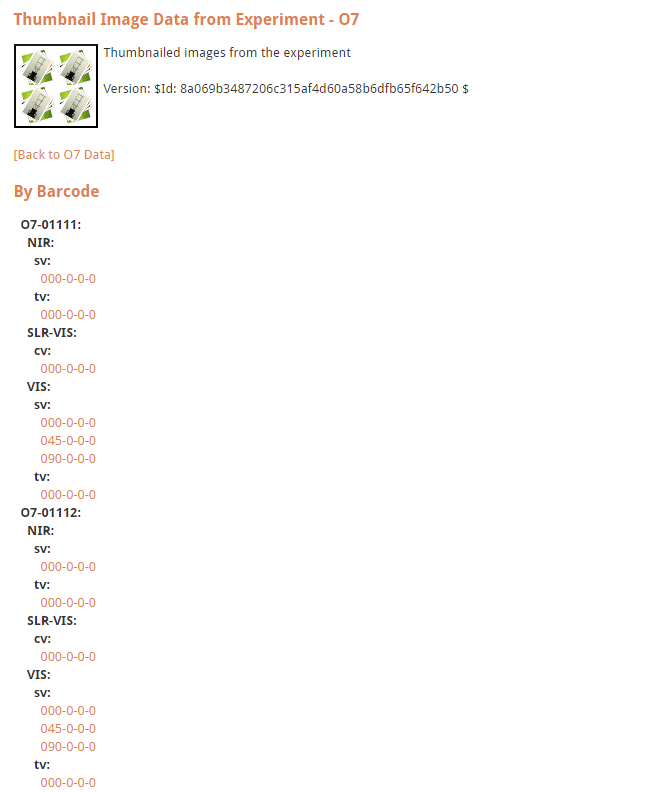
\includegraphics[width=0.7\textwidth]{images/background/access_phen}
    \caption{Current means of NPPC image exploration}
    \label{fig:acc_phe}
\end{figure}

The second existing solution investigated is a commercial product called Zegami\cite{_Zegami} developed in part by Oxford University. Figure~\ref{fig:zegami} shows the Zegami system in action on the Australian Plant Phenomics Facility\cite{_aus} website. Zegami is a web based tool that allows the browsing of large amounts of images in a fairly intuitive and responsive way and also provides the means to search, sort and filter images using associated data attributes. Zegami allows the visualisation of data in graphical formats and provides the means to select subsections of the images based on selections made in the graphical views via drawing boxes or circles around the desired datapoints.

Being positioned as a image and data exploration tool, data addition is mostly done from a single datasource file in Zegami with no out-of-the-box facility for users to add supplementary data to an experiment.

Zegami is a feature-rich and robust solution for exploring large collections of images and associated data, however, being a commercial venture it is not free and can be considered prohibitively expensive a solution for a project of this nature.


\begin{figure}[H]
    \centering
    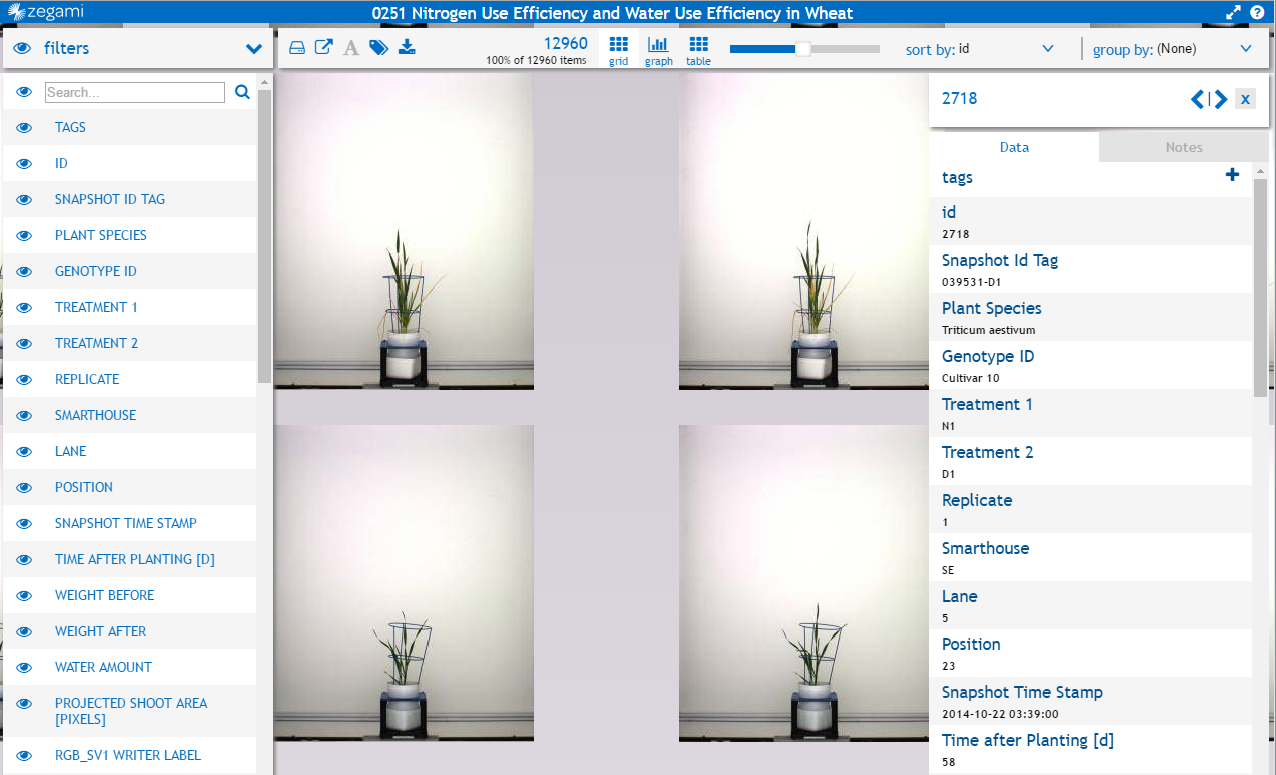
\includegraphics[width=0.7\textwidth]{images/background/zegami}
    \caption{Zegami system as used by the Australian Plant Phenomics Facility. Source : \url{https://zegami.plantphenomics.org.au}}
    \label{fig:zegami}
\end{figure}
\section{Analysis}
%Taking into account the problem and what you learned from the background work, what was your analysis of the problem? How did your analysis help to decompose the problem into the main tasks that you would undertake? Were there alternative approaches? Why did you choose one approach compared to the alternatives? 

%There should be a clear statement of the objectives of the work, which you will evaluate at the end of the work. 

The core problem that this project aims to solve is the need for a web-based system that enables the exploration of images and associated data that are collected during experiments at the NPPC. 


 Following the domain research and familiarisation with the NPPC gained during the discovery period for the initial project specification it was felt that the new direction of the project was well understood and that certain requirements could be identified fairly quickly. The following list will detail these and further additional requirements identified during the course of the project to provide a complete view of targeted functional specifications.


\subsection{Requirements decomposition}

%In most cases, the agreed objectives or requirements will be the result of a compromise between what would ideally have been produced and what was felt to be possible in the time available. A discussion of the process of arriving at the final list is usually appropriate.

\subsubsection{Web based system} In order to provide a practical solution to the problem, access to the system should be available from a wide array of devices and systems. The system should also be accessible from a variety of different locations. The most practical solution to these considerations is a web based approach. Most devices and systems natively support some kind of web access and a centrally hosted solution is far more accessible than any alternative approach.


\subsubsection{Integrate with NPPC data repository} The system needs to display plants, plant images and associated data. Data and images captured at the NPPC during experiments are stored in a central data repository hosted on the Aberystwyth University network. In order to provide access to these images and data via a web based approach, it is necessary to integrate the system with the data repository such that the images or data can be pulled directly from the repository as opposed to re-hosting the same content within the delivered system itself. The sheer quantity of image data in the repository itself makes a re-hosting solution highly impractical. 

 
\subsubsection{Browse plants and plant images}  Users will be able to view plants, associated data and plant images. In order to provide a means of exploring the data and images captured at the NPPC, the system needs to provide some interface onto these data that allows easy navigation between plants, images and associated data. Currently there is no consolidated interface onto both experiment images and the data observations captured during the course of experiments. Providing such an interface makes the exploration of past and current experiments convenient and simple.

\subsubsection{Import experiment data}  Experiment data will be imported into the system from file and associated with the plants in an experiment. The biologists conducting experiments will invariably use spreadsheets in order to capture observations and data on plants in the experiments. The system needs to be able to incorporate these data with minimal manual processing such that the system can be used to link these data to the plant images. 

\subsubsection{Add meta data to plants and plant images}  Users will be able to add supplementary data to individual plants and images. In order to provide the opportunity to supplement experiment data with further information, a facility to add data to the system is required. The addition of data in this manner allows the creation of richer, more complete datasets for a given experiment with potential for future use in other applications and analyses. 

\subsubsection{Persist data in local database} Image data is sourced directly from the NPPC data repository. Data imported or input into the system needs to be stored in a persistent way. Access granted to the NPPC data repository is read only for security and data integrity purposes. A database local to the delivered system provides a solution that allows fast queries of contained data, avoiding any network over heads, and provides the means to store experiment and supplementary data. Exports can potentially be taken from the database in order to migrate the data to a separate system or facilitate its use as a dataset for future work. 

\subsubsection{Display graphs of data in system}  Visualising the data within the system is key to facilitating the quick understanding and digestion of captured data. Using graphical visualisations provides the means of quickly comparing certain data attributes or deducing whether there are interesting correlations or outliers in the data. Graphical visualisations can be used in order to quickly determine whether further statistical analysis of subsets of captured data is worthwhile or likely to produce interesting results. Providing the means to quickly create arbitrary visualisations from the experiment data allows the experimenters to see the data in ways that would previously require a much larger degree of manual effort.

\subsubsection{Administrator panel or page to manage the system}  A means of managing the experiments in the system will be provided via a web page with restricted access.








\subsection{User Roles}
For this system there were two identified user roles, an administrator or admin role and a general user role.

\subsubsection{Admin}

Figure~\ref{fig:admin_case} shows a use case diagram for the admin user. The admin manages experiments in the system with the facility to initialise new experiments or delete previously initialised experiments. The admin user can also manage the data associated with an experiment by importing experiment data from file or resetting the data associated with the experiment back to its newly initialised state.

\begin{figure}[H]
    \centering
    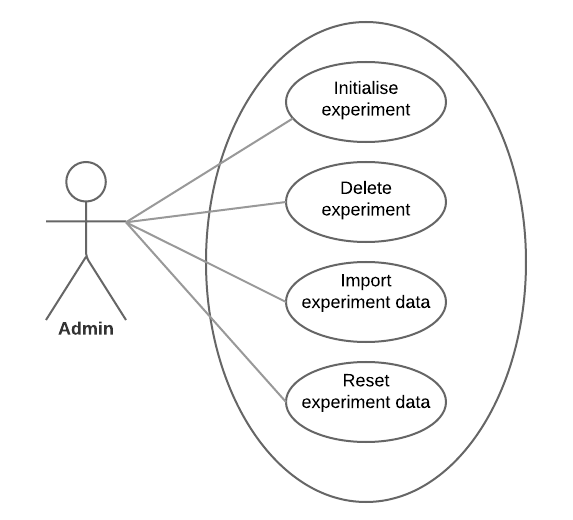
\includegraphics[width=0.5\textwidth]{images/analysis/admin_case}
    \caption{Use cases for admin user}
    \label{fig:admin_case}
\end{figure}

\subsubsection{User}

Figure~\ref{fig:user_case} shows the use cases for the general user role. Users of the system are able to select between the various available experiments and browse the plants and images associated with them. Users are able to add data to plants in the form of tags or key value pair attributes. Users are able to generate graphs from the available data.

\begin{figure}[H]
    \centering
    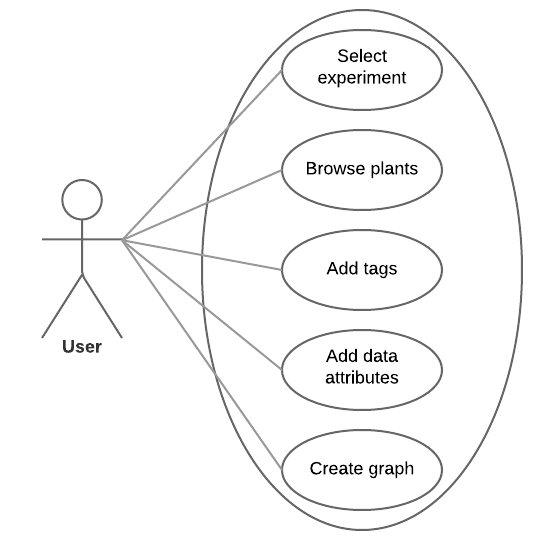
\includegraphics[width=0.5\textwidth]{images/analysis/user_case}
    \caption{Use cases for generic user}
    \label{fig:user_case}
\end{figure}

\section{Process}

Plan driven approaches traditionally associated with software development projects usually expect that all system requirements are understood and collected prior to any further work on design or implementation. A number of factors made such an approach unsuitable for this project, chiefly a lack of domain knowledge made up-front requirement gathering difficult and the requirements themselves were likely to be poorly defined and subject to change. 

The methodology used for the delivery of the project was an agile approach based on the popular SCRUM methodology. For the duration of the project, work would be carried out in time-boxed iterations or `sprints', each a week long. Sprints would begin with a planning session and end with a release of the system software. At the conclusion of each sprint a short retrospective analysis of the sprint would take place, looking at what went well and what could improve for the next iteration. The focus on incremental delivery of working software allowed the project to evolve in an emergent fashion whilst remaining continuously functional as features were prototyped, designed and implemented.  

System requirements were broken down into user stories which in turn were broken down into individual tasks if necessary. As in SCRUM, these stories were held in a backlog until being added into a current or future sprint depending on priority and the goal for a particular sprint. Emergent issues such as priority bugs could easily be incorporated into the wider context of the current sprint if necessary which allowed work to be focused on the most pressing issues. The Jira \cite{jira} issue tracking application was used in support of this process providing an environemnt in which to specify and track user stories,task and sprints, see section~\ref{jira_sec} for further details. 

During a sprint, each day would begin with a quick overview of tasks in the sprint, replicating the `stand-up' meetings common in SCRUM. Work would be commenced or continued on the task deemed highest priority at the time. At the end of each day a short update would often be posted on the project blog available at \url{https://siongriffithsblog.wordpress.com/} summarising the days activity. The blog itself has proven to be a useful part of the process, helping to document certain aspects of the implementation and design that may have otherwise been forgotten.


\subsection{Time Management}
Effective management of time is a key consideration of any reasonable development process model. Partway through the project it was decided to fully adopt the Pomodoro technique \cite{pomodoro}, working in blocks of twenty five minutes with complete focus on the task at hand, referred to as Pomodoros. A five minute break is taken after each successful twenty five minute work block in order to avoid the mental fatigue of attempting to remain focused and productive for an extended amount of time. Taking these regular, short breaks allowed for a higher degree of productivity over the course of a work day.

Having distinct blocks of time in which to complete work compliments the SCRUM approach to effort tracking and estimation. Although not part of the initial process, towards the latter half of the project after gaining a sufficient feel for the possible output of a single Pomodoro, all work was estimated in terms of the Pomodoros required to complete the task. The goal for a given sprint was to achieve sixty Pomodoro and use this figure as the budget for work that could be done. It was fairly difficult to estimate in terms of Pomodoro and often fairly inaccurate, although the productivity aspect certainly works, the more abstract and popular `story-point' method of effort estimation is what would be used if the project was repeated.

Figure ~\ref{fig:pomo1} shows the early Pomodoro tracking during two iterations. A successful Pomodoro would result in a sticker being allocated to that day. It was preferable to have Pomodoro goals for a given sprint rather than concrete work times (for example nine-to-five) since this allowed a great deal of flexibility whilst also maintaining that a weeks worth of work was to be done. Effort could be expended in the beginning of the week in order to have more time later on for example.  

\begin{figure}[H]
    \centering
    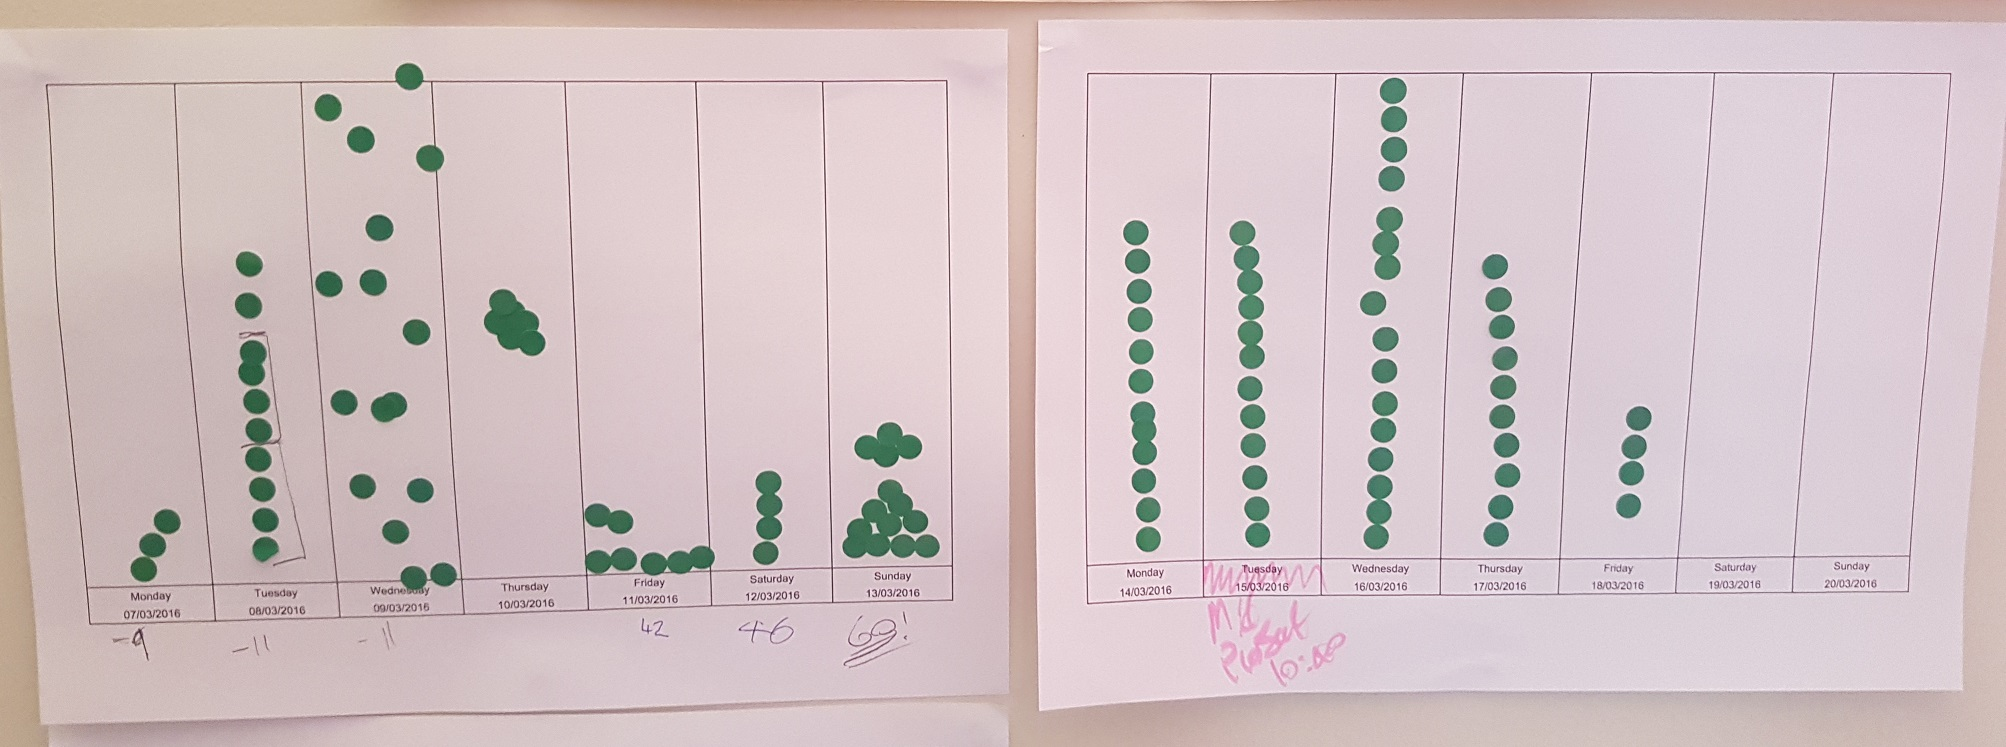
\includegraphics[width=\textwidth]{images/process/pomotrack}
    \caption{Tracking pomodoros}
    \label{fig:pomo1}
\end{figure}


%The process used for the project was an agile based approach similar in style to Scrum although adapted for a project team of one. The process centred around User Stories and short iterations of one week. 


%\addcontentsline{toc}{chapter}{Development Process}
\chapter{Design}

\section{Overall Architecture}\label{arch}

The overall architecture of the system can be described as a mixture of two well known architectural patterns, Model View Controller(MVC) and 3-tier architecture. 

\subsection{MVC}\label{sec_mvc}

The Model View Controller paradigm is synonymous with web application development these days and is often employed without much consideration for alternatives. The fact is that the MVC pattern is so ubiquitous and well supported and understood that it is difficult to make a case against its use for a project of this nature, where MVC fulfils all expectations for a data driven front end to a web application. Many of the alternative approaches share the same primary goal as MVC, seperation of concerns, keeping the display and data components separate. However these alternatives lack the penetration that MVC currently has and as such their comparative obscurity makes them less desirable from a general maintenance point of view since it can be expected that a greater number of developers will already be familiar with MVC. Many mature and well maintained frameworks offer MVC as default out of the box in a well supported and easy to understand manner, for these reasons not much consideration was given to other possible solutions although some were briefly looked at.

Figure~\ref{fig:mvc} provides a high level overview of the way in which the MVC pattern is structured. For this project, each web page will be represented as its own view with its own dedicated controller, providing a high degree of modularity and helping to keep the individual controller classes thin in order to aid code navigation, maintainability and scalability of the solution. 

\begin{figure}[H]
    \centering
    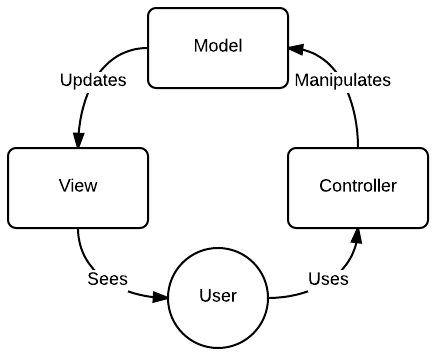
\includegraphics[width=0.5\textwidth]{images/design/mvc}
    \caption{Model View Controller pattern overview}
    \label{fig:mvc}
\end{figure}


\subsection{3-tier Architecture}
The second architecture pattern making up the system design is 3-tier architecture. The goal of the 3-tier pattern is to separate the system into 3 distinct, modular tiers. These layers are the presentation layer, the business logic or service layer and the persistence layer.  

In this project the presentation tier encapsulates the entirety of MVC pattern described in section~\ref{sec_mvc} above, the MVC controller for a particular view will make a request to a service layer class and use the resulting data to populate a model for returning to the view.

 The service layer is where the business processes are carried out. Logical processes, data transformations and calculations are all carried out within this tier. The service layer also acts as a go-between for the presentation and persistence layer, translating requests and results into compatible forms for the other tiers.
 
 The persistence layer, or data layer, is concerned with data storage and retrieval, usually, and for this project entirely, from a database system. All crud operations and queries on database entities are performed within this layer allowing the service layer and its containing logic to be abstracted away from the database.
\begin{figure}[H]
    \centering
    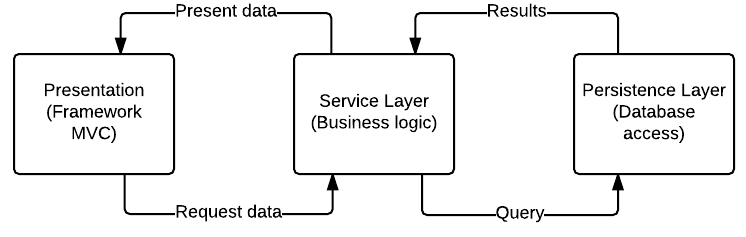
\includegraphics[width=\textwidth]{images/design/3t}
    \caption{3-tier architecture overview}
    \label{fig:3t}
\end{figure}

The 3-tier pattern is a useful design within this project because it allows modularised and compartmentalised code to be written and maintained. Using the 3-tier pattern allows a developer to modify one of the distinct layers without having to rewrite the entire system. For example, all the queries and database calling methods could be changed to use totally different technologies and provided the same hooks are available for the service layer to gain access then the system would function as expected with no modification to service or presentation layers. Figure~\ref{fig:arch1} shows the relationship between layers using a subset of the system components. Service layer dependencies are wired into each controller that require access to the processes in that service or the data in the database access object (Dao) coupled to a given service. 

\begin{figure}[H]
    \centering
    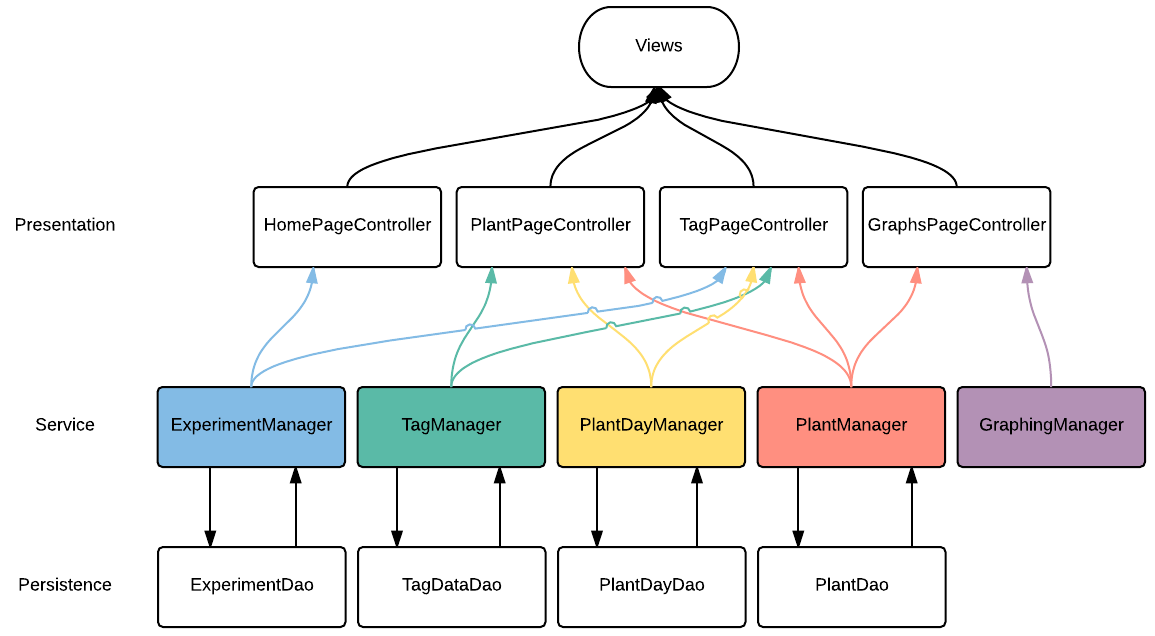
\includegraphics[width=\textwidth]{images/design/arch1}
    \caption{Architecture and dependency wiring}
    \label{fig:arch1}
\end{figure}

\section{Framework and Programming Language}\label{framework}

The sheer range of MVC frameworks available to developers is incredible and the decision of which to use is potentially difficult. It was not within scope to review a large amount of potential choices and to research which were mature, well supported solutions rather than a `flavour of the month' framework. The two main contenders considered for this project were Ruby-on-Rails and the Java based Spring. Both are mature, well supported technologies with a large range of compatible libraries. Both have large and active communities surrounding and supporting them and both have well maintained official documentation. Both have convenient front-end templating technologies. Both share a  `convention over configuration' approach and importantly both are capable of supporting the designs discussed in section~\ref{arch}.

For the purposes of this project, Spring was eventually selected. Specifically the Spring Boot\cite{_boot} bundle which greatly reduces initial configuration time at the start of a project and allows simple integration of complex packages (such as the Spring-Data package discussed in section~\ref{db}) via so called `starter' packages. External dependencies are minimal and the system can be run on a wide variety of hardware configurations without the need to rebuild. 
 Even though both frameworks offer inversion of control and dependency injection, the annotation based Spring approach is preferable, especially when coupled with a fully featured IDE capable of understanding the wired dependencies and annotations. 

Using a framework based on Java has some arguable advantages, the fact that Java is compiled provides an extra level of checking during development and provides a quick notification of overlooked errors that may take time to uncover in an interpreted environment such as that provided by Rails. Java has built in security and type-safety providing peace of mind both in guaranteed resolution of variable types and built in access control at the virtual machine level. 

Initially the project was developed using the latest version of Java (version 8), however, in order to take advantage of the available hosting environment at the NPPC it was necessary to use version 7 as this is what was installed on the systems. Fortunately the change was relatively straight forward since  much of the work carried out prior to this 





\section{Domain modelling}

Designing a domain model representation for the project was fairly straight forward. It was clear from initial investigations that a simple relationship existed between the primary domain entities that were going to be represented by the system. Essentially, there are Experiments, Experiments have a number of Plants associated with them and these Plants never belong to more than one Experiment at a time. Each Plant then has a number of images associated with it. There is a clear one to many relationship between these entities that is intuitive and can be modelled easily.

Further consideration of this domain model design following some initial implementation led to the inclusion of the PlantDay class in order to better represent the time serried nature of the images and data associated with a Plant. The Plant class now has many PlantDays which has many PlantImages. Each unique date that has images of a Plant is represented as a PlantDay. PlantImages with the same date are grouped together within the same PlantDay. This gave rise to the final design for the relationship between these domain entities, figure~\ref{fig:domain1} shows how this relationship is modelled within the system. 


\begin{figure}[H]
    \centering
    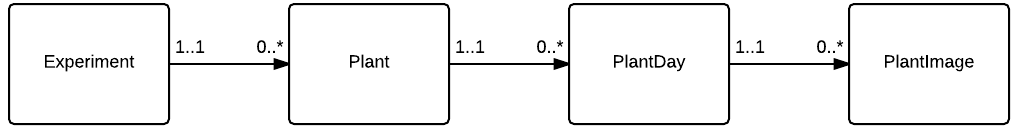
\includegraphics[width=\textwidth]{images/design/domain1}
    \caption{A simplified class diagram showing the relationship between primary domain entities}
    \label{fig:domain1}
\end{figure}


Having modelled the entities in the system, consideration was given to the best approach to adding data to the entities. There are two primary modalities to the data expected within the system, data directly associated with a top-level Plant and time-serried Plant data which would be associated with a date or PlantDay. After investigating different examples of data collected during experiments it was decided that there would be two primary data classes. A Metadata class which would hold a map structure and share a one-to-one relationship with unique Plants and PlantDay instances, and a TagData class which would be unique to the tag content it contained and potentially referenced by many Plant or PlantDay instances.

Since it was clear that experiment data is possibly very different from one experiment to the next, the system had to be permissive in how the data is associated with domain objects. Arbitrary attributes and values had to be supported and this is why the approach with the Metadata class is to have a map structure holding string values for attribute key/value pairs. Using strings meant that both numerical and text data could be represented within the same structure, leaving conversion and/or checking requirements to other parts of the system if required. This was deemed acceptable since for the most part the system is only storing and displaying these data rather than using the values directly for calculations for example. Both the Plant class and PlantDay could have held the metadata map as instance variables, and indeed they did initially, but it became apparent that porting it out into a single class would enable the data to be queried natively on the database (discussed further in section~\ref{db}) and cut down on the number of unique queries required in the Java code in order to find metadata instances.

Whilst the Metadata class represents general experiment data for each Plant and PlantDay, the TagData class was designed to hold sparsely associated data. The majority of Plants would be untagged, tags are used as supplementary comments against the occasional Plant to note some interesting information (common examples seen were `dead' or 'small'). The approach with the TagData class was to have a unique instance for each unique tag, for example, all Plants with the tag `dead' shared a reference to the same tag instance with content `dead'. This provided a simple way to enable returning all Plants sharing a tag within an experiment via queries against the content of the associated TagData. Figure~\ref{fig:domain2} shows the complete relationship between the domain model classes. Essentially these classes are all Plain Old Java Objects (POJO) which is why such a simple diagram suffices, the methods they contain are all getter/setter type methods and can be omitted from the relationship diagrams.


\begin{figure}[H]
    \centering
    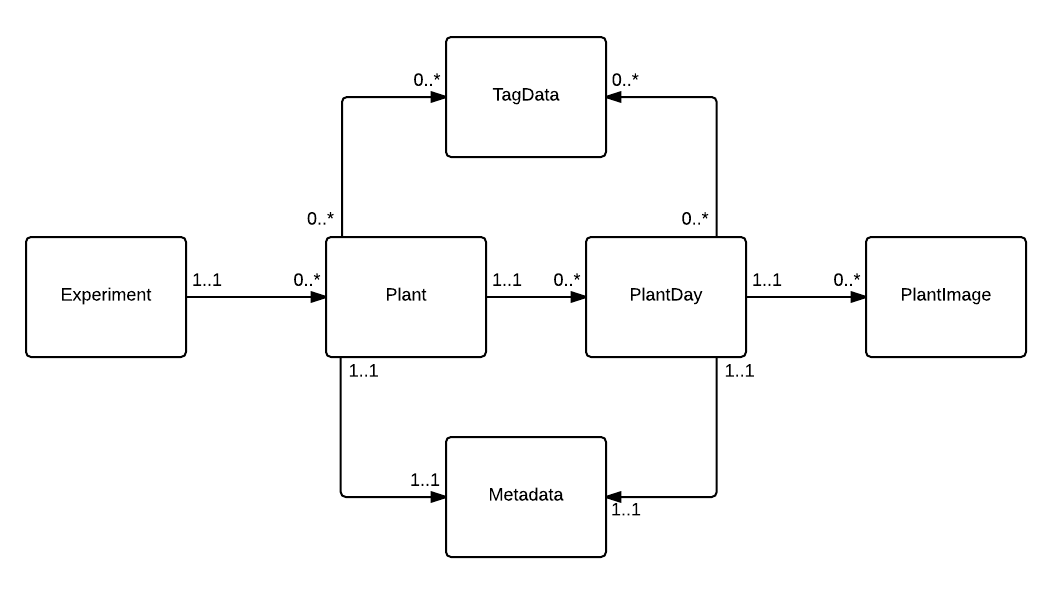
\includegraphics[width=\textwidth]{images/design/domain2}
    \caption{A simplified class diagram showing the domain model}
    \label{fig:domain2}
\end{figure} 

\section{Database} \label{db}

For this project the database structure is entirely derived by the Hibernate\cite{_hibernate} object relational mapping (ORM) which is included in the Spring framework within the Spring-Data project as part of its Java Persistence API (JPA) support. The ORM system allows a developer to annotate Java code with keywords that inform the ORM system of how to represent a given class and persist it in the database. This technique allows the developer to manage the persistence element of a system from within the same object-oriented paradigm that the rest of the system is written in. It provides a level of abstraction away from the managing of the database itself leaving the developer to define only the structure of the data rather than its precise representation within a specific database system.

 Listing~\ref{lst:orm} shows an example of these annotations within the Plant class. The class is annotated with \texttt{@Entity} to inform the ORM that it is a managed class to be persisted and table constraints are declared. The getter methods for the instance variables in the class are annotated with relationship definitions if applicable, including foreign key mappings and what manner of database instructions should cascade through the relationship to the related entity. The annotations can also define a fetch type which can take the value \texttt{LAZY} or \texttt{EAGER}, this defines whether the related entity objects should be fully initialised when the parent is called or whether, in the case of a \texttt{LAZY} fetch, a proxy object with no instance variables initialised should be returned. For this project, the use of \texttt{LAZY} fetch is preferred in all situations since it allows greater control over the performance of the system. If for example, the Plant class made an eager fetch for it's associated list of PlantDay objects, each PlantDay would be fully initialised at the time when the Plant object is retrieved from the database via a query, resulting in extra queries to the database in order to fully populate each PlantDay. Using this fetch technique allowed the PlantDays to be initialised when a method like \texttt{.size()} was invoked on their containing list or a getter method was invoked on the PlantDay itself. 

\lstjava
\lstinputlisting[label={lst:orm},caption=Detail of ORM annotation in Java class]{sourceCode/mySnippets/design/plantorm.java}

Figure~\ref{fig:dbSchema} details the database schema resulting from the ORM annotated relationships within the system. As discussed previously in this section, the relationships are a direct result of the structure of the Java code and the choices made with certain annotations, such as which side of a relation should hold a reference to the other.

 The main deliberate change made to the default ORM mapping onto the database was to pull the dataAttributes map (a \texttt{Map<String,String>} representation in Java) out from the Metadata object into its own table, `metadata\_data\_attributes'. The default would have been to map this as a blob type column within the metadata table, however, in order to ensure that all data within the database can be queried via native queries on the database itself, this extra table approach was taken.


\begin{figure}[H]
    \centering
    \includegraphics[width=\textwidth]{images/design/dbSchema}
    \caption{An entity relationship diagram for the database schema}
    \label{fig:dbSchema}
\end{figure}

From a developer based standpoint, when using an ORM such as the Hibernate system provided in Spring, the underlying database technology is mostly transparent. Provided the database is of a type supported by the ORM, the developer need not make any changes to the code in the system in order for the underlying database technology to change. Custom queries implemented within the system are defined using JPA syntax and are abstracted away from the underlying database. However, consideration was given to the database system to ensure that the best choice was made both to support efficient representation and to ensure compatibility with a wide range of possible hosting environments and potential future maintenance needs.

It was clear from very early in the project that the data to be persisted within the system had structured relationships between entities which favours the more traditional SQL type databases over NoSQL solutions. It is forecast that the increased scalability offered by a NoSQL solution would not be required for this system, traditional SQL management systems are capable of scaling up to many millions of entries which should be more than sufficient for this system. With this in mind a MySQL solution was chosen, it is widely supported and well understood in terms of potential maintainers along with being a default technology on many operating systems including the hosted environment provided for the system.

\section{Data Import}

When designing the data import system the primary objective was to try and preserve, as much as possible, the format and structure of the original data files produced as part of an experiment. Figure~\ref{fig:data1} shows an excerpt from a spreadsheet provided as an example of real experiment data. 

\begin{figure}[H]
    \centering
    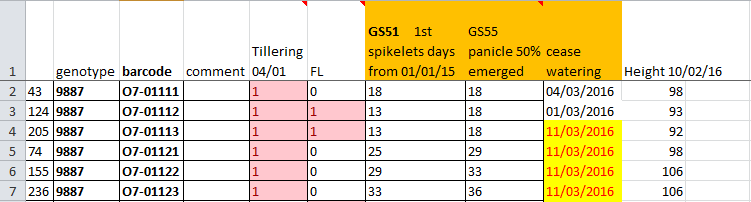
\includegraphics[width=\textwidth]{images/design/data1}
    \caption{A sample of provided experiment data in its original form}
    \label{fig:data1}
\end{figure}

For representing these data, the CSV format is the obvious choice and is available as one of the default export options for spreadsheet applications. The design challenge was routing the data from the CSV file into the system whilst enabling arbitrary values for identifiers to allow for the vast potential range of different data to be captured by the system. However, the format of the files needed to change as little as possible to simplify the use of the system and to minimise the amount of work required on the data to get it ready for import.

The solution was to use a simple annotation based method to identify how each column of the CSV should be routed. Listing~\ref{lst:annot} shows how these annotations are represented and used within the header of the csv file. 
\begin{lstlisting}[label={lst:annot},caption=Excerpt showing annotated CSV header for data import]
{{plant-a}}genotype,{{bc}}barcode, {{plant-t}}comment,{{day-a}}Growth Stage~~51,
\end{lstlisting}
There are four supported annotations:
\begin{enumerate}
\item \textbf{\{\{bc\}\}} - Identifies the column as the barcode for a Plant. This serves to uniquely identify the Plant to which the data in the row should be assigned.
\item \textbf{\{\{plant-a\}\}} - Identifies the column as a Plant attribute. The content of the header column is used as the identifier and the content within the row is used as value. 
\item \textbf{\{\{plant-t\}\}} - Identifies the column as a Plant tag. The content of the header column is ignored and the content of the row is added as TagData to a Plant.
\item \textbf{\{\{day-a\}\}} - Identifies the column as a PlantDay attribute. Uses a specific delimiter token \verb|~~| in order to split the header column into a key value pair. The column in the row in this instance needs to be a date such that a specific day can be allocated the data.
\end{enumerate}

Other methods investigated included using XML and JSON within the CSV to identify certain fields in the header and columns. However, even though both XML and JSON are convenient ways to represent and parse semi-structured data, they are not particularly quick to use in terms of the characters needed to be typed and neither are they especially readable when crammed into the header of a CSV file. In keeping with the goal of simplicity these alternatives were quickly discounted in favour of the simple annotation method. 

\section{UI}
The UI design process used within the project is fairly straight forward and relatively basic. Essentially the process used would first involve a wire frame mock up of the page, an example for the Plant Detail page is shown in figure~\ref{fig:ui1}. This would then be prototyped and the design would evolve iteratively as implementation proceeded and user feedback testing was conducted.

\begin{figure}[H]
    \centering
    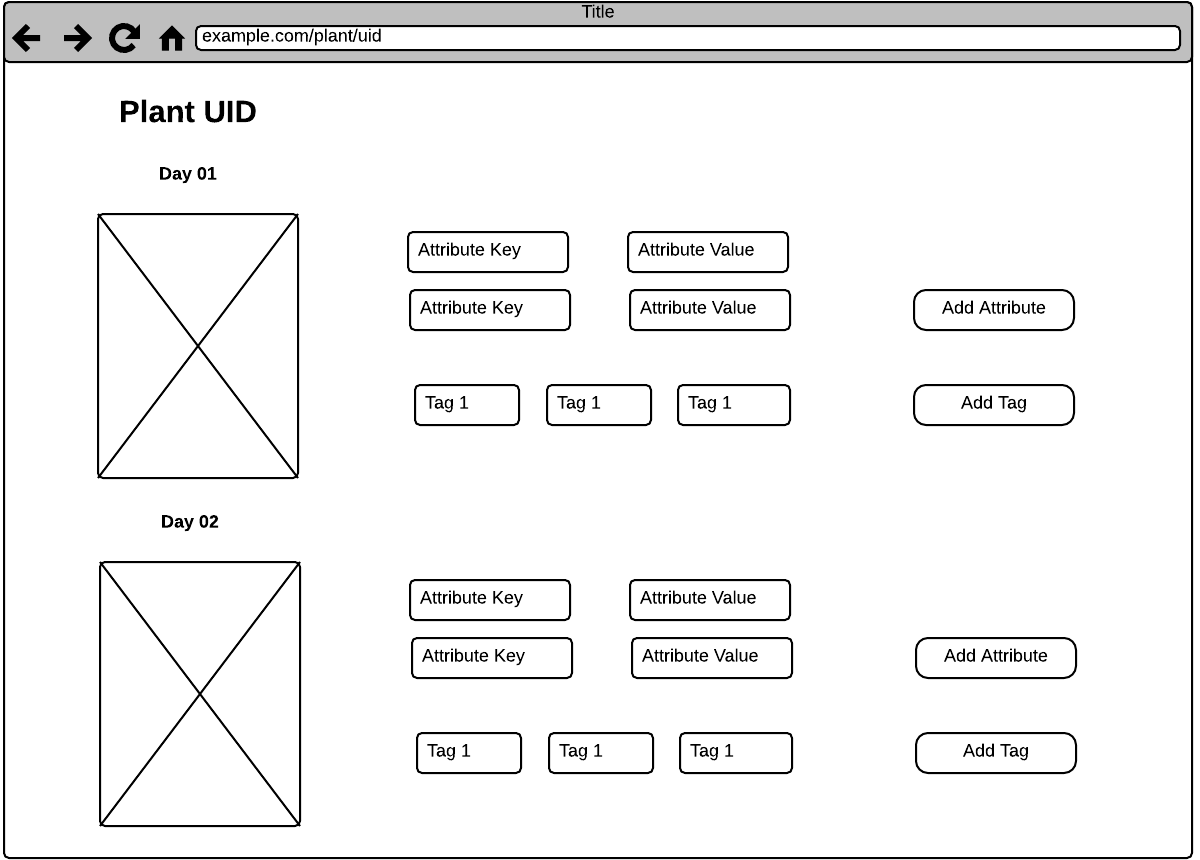
\includegraphics[width=\textwidth]{images/design/ui1}
    \caption{An early wireframe design for the Plant Details page}
    \label{fig:ui1}
\end{figure}

Figure~\ref{fig:ui2} shows the final look of the Plant Detail page, it's clear to see how it relates to the initial wire frame and also where implementation decisions have resulted in some minor tweaks to the design. This same process was followed for all the pages within the system, where the focus has been on a simple yet usable design with minimal clutter. 

\begin{figure}[H]
    \centering
    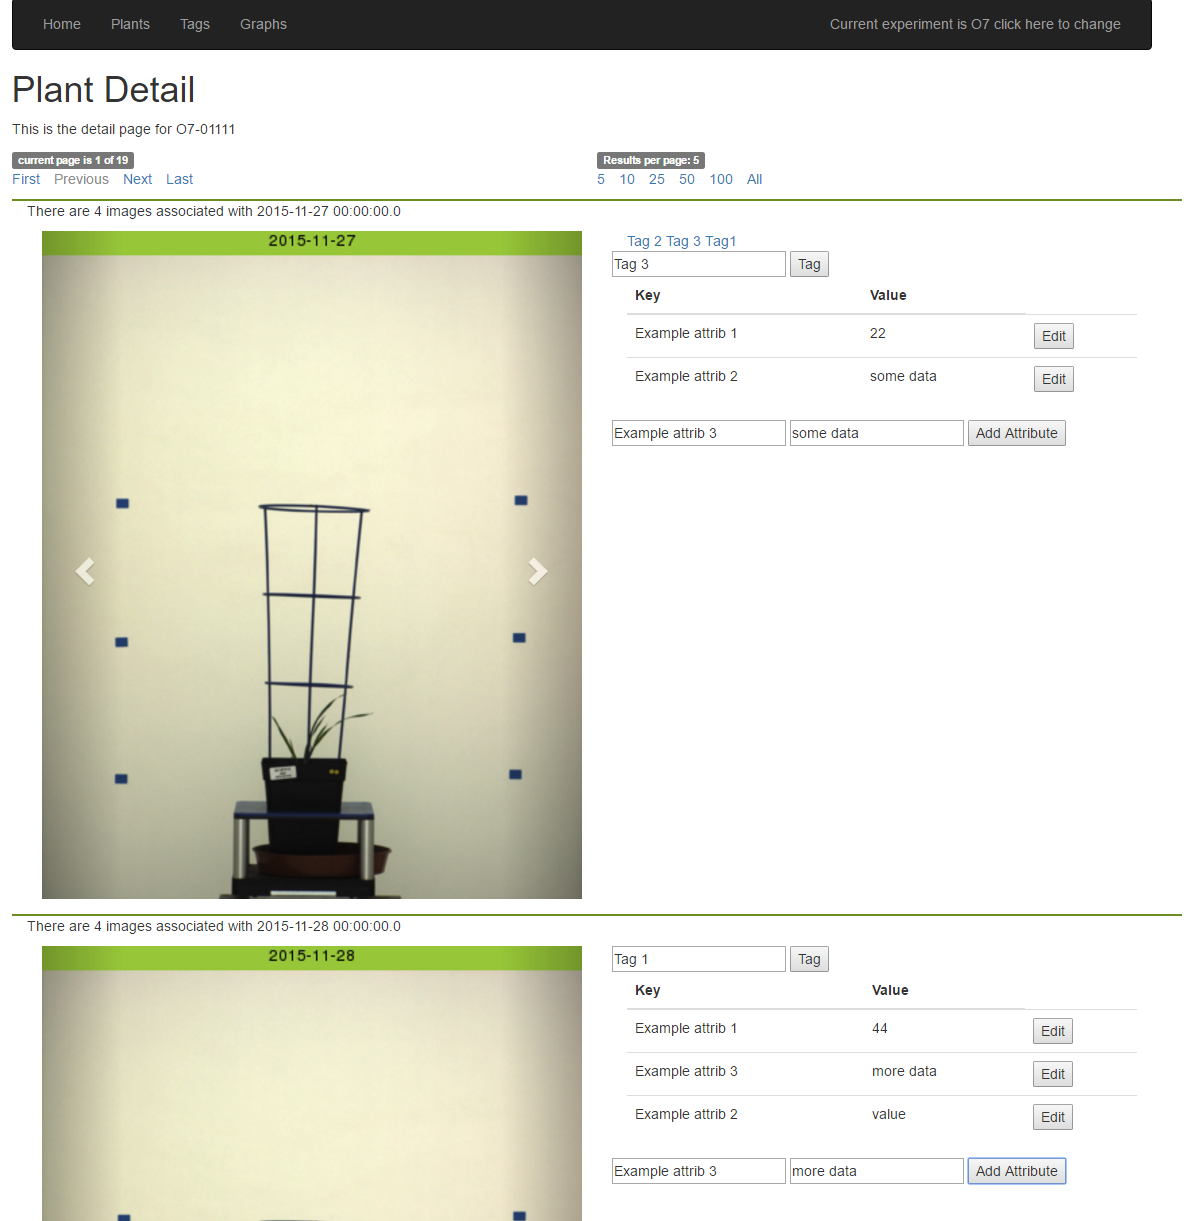
\includegraphics[width=\textwidth]{images/design/ui2}
    \caption{A screen shot showing final design of Plant Details page}
    \label{fig:ui2}
\end{figure}

A design consideration for UI interaction was that user interactions within a page should always use an asynchronous method to update the page with results of the interaction, such as crating a graph, tagging Plants or editing attributes. This asynchronous approach was achieved via the use of ajax based javascript functions invoked when users would click buttons or links. The view controller class within the framework would process these ajax requests and return the HTML for a partial page fragment which would then be injected back into the page in order to provide updated content without the need of a page refresh.

\section{Tools and third-party services}
\subsection{Intellij}

Intellij \cite{_intellij} is the core development tool used during the completion of this project. It is a fully featured Java integrated development environment (IDE) that has support for a wide range of features including Spring and Github (see section \ref{gitsection}) integration right out of the box. Its code completion and debugging tools are significantly more refined in comparison to the most popular alternative Eclipse, allowing for faster writing of code and easier debugging. As with any reasonably modern IDE, IntelliJ comes with the facility to run sophisticated test suites, providing code coverage metrics and providing auto-generated method stubs in implementation or test classes further speeding up development time, especially in boiler-plate heavy languages such as Java.

IntelliJ also provides in-built static analysis tools that run automatically has part of committing changes to version control via the IDE. This is useful as it is configured to highlight warning level issues which include code style along with potential logical mistakes within sections of code and even spelling errors. Having these checks at commit time enables the developer to review any potential problems before the code gets checked into the repository, although the results are often a little too pessimistic they are still useful. Figure \ref{fig:intellij} shows the IntelliJ IDE with static analysis results displayed.

\begin{figure}[H]
    \centering
    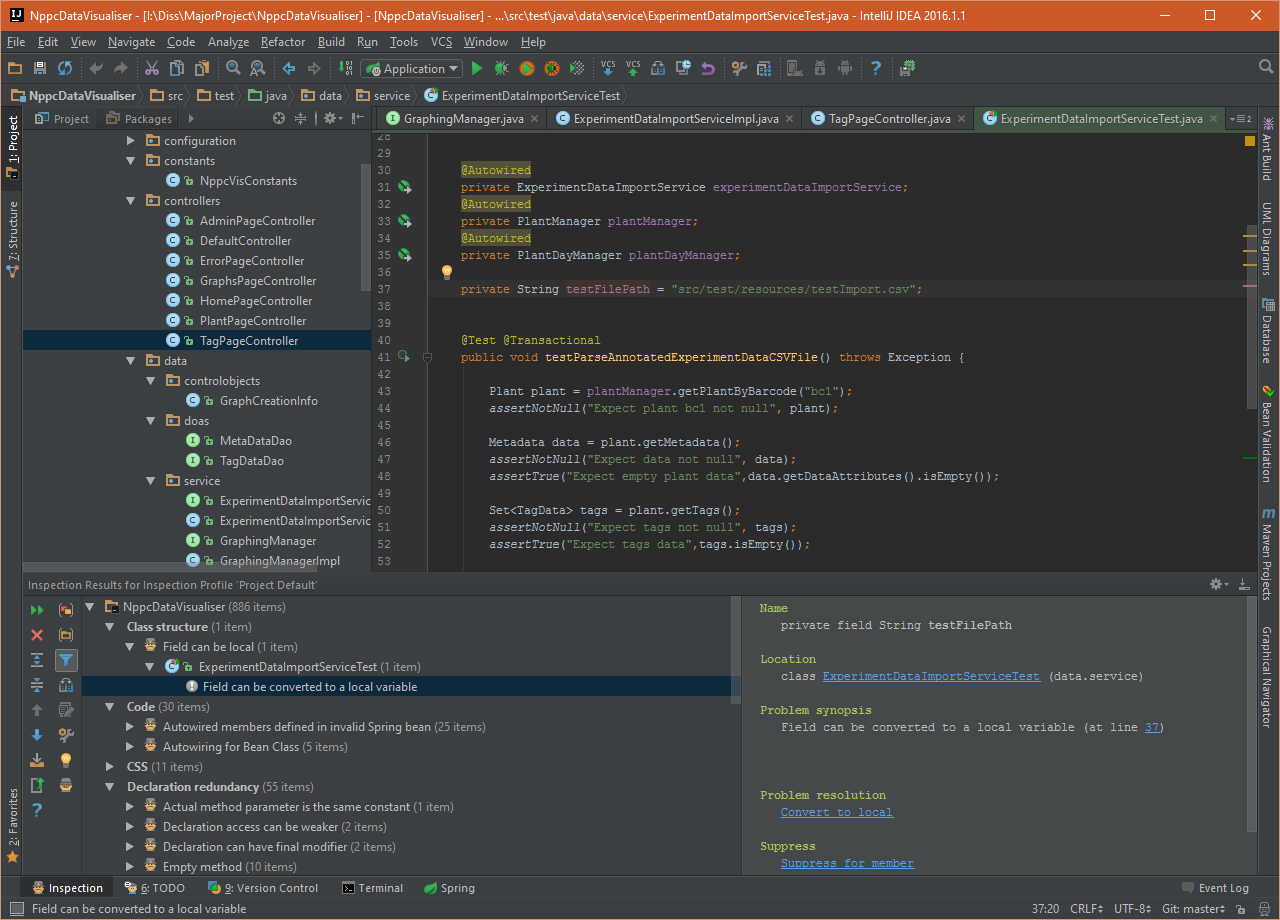
\includegraphics[width=\textwidth]{images/tools/intellij}
    \caption{The IntelliJ IDE showing result of static analysis}
    \label{fig:intellij}
\end{figure}

\subsection{Git and Github} \label{gitsection}

The use of version control is invaluable in modern software development. It has become a necessity in even the smallest of hobby projects since it allows the developer to be confident in making changes without having to worry about rescuing previous version if things go wrong and provides development teams with the means to work concurrently and collaboratively on the same code base. 

The version control system selected for this project was Git \cite{_git}, having previously used alternatives such as Subversion I chose Git for its integration with more numerous, modern services and the fact that it allows local copies of a repository which is synced with a remote repository as opposed to the remote-only approach taken by Subversion.

The Git repository for this project is hosted on Github \cite{_gitHub}, a web based service dedicated to providing git repository hosting and related facilities, such as commit history tracking, release visioning and integration with third party services. There are alternatives to Github available but due to familiarity brought on by hosting all previous projects and the fact that Github is now an industry leading solution, it was decided to use Github for this project without any real evaluation of alternatives since it was well known that Github could provide all facilities required for the purpose of this project. Figure \ref{fig:gitrel} details one of the tagged release versions of the system within Github. Having releases tagged in this way allows easy rollbacks to previous release versions in the event of any major issues in a new release. 

\begin{figure}[H]
    \centering
    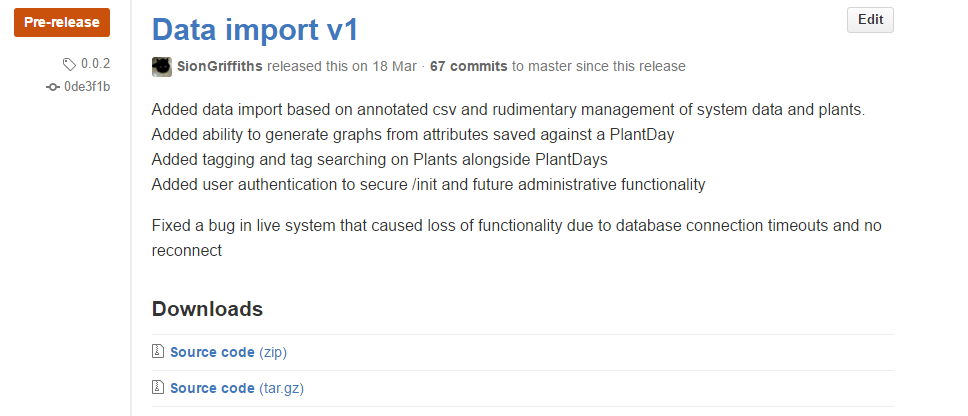
\includegraphics[width=\textwidth]{images/tools/gitrel}
    \caption{A tagged release of the project within Github}
    \label{fig:gitrel}
\end{figure}

\subsection{Jira} \label{jira_sec}

Jira \cite{jira} in an issue tracking and project management tool provided by Atlassian, an Australian software company. It is an industry leading product used by many companies for tracking their projects and the issues within them. Its use on this project was in support of the agile approach to project development, allowing the specification of user stories, development tasks and their inclusions within configurable sprints or development iterations. Figure \ref{fig:jira_sprint} shows the current sprint view in Jira, user stories are grouped into `lanes' corresponding to their status, allowing a simple way to track the work completed and left to do within in the current development iteration.

\begin{figure}[H]
    \centering
    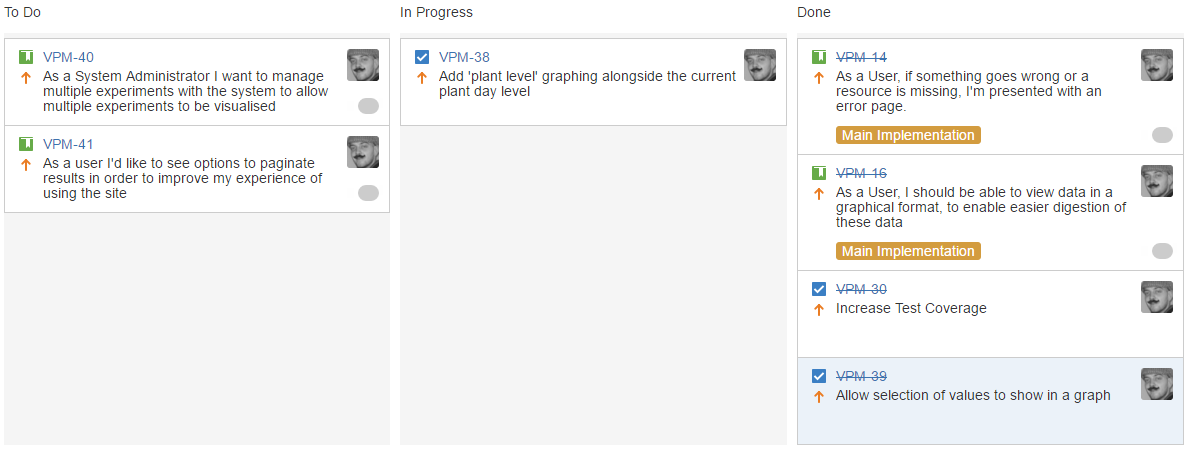
\includegraphics[width=\textwidth]{images/tools/sprint1}
    \caption{Current sprint screen in Jira}
    \label{fig:jira_sprint}
\end{figure} 

 Bugs could also be tracked as issues within Jira and added to the current sprint if necessary, I found this to be a valuable way to deal with emergent issues during development as it allowed a simple way to assign priority to urgent issues and keep track of less usgent bugs in the project backlog to be worked on in a future sprint. Figure \ref{fig:jira_bugs} shows a selection of bugs raised as part of development, Jira provides simple methods for filtering all issues against a project by type or status allowing quick access to screens such as this.

\begin{figure}[H]
    \centering
    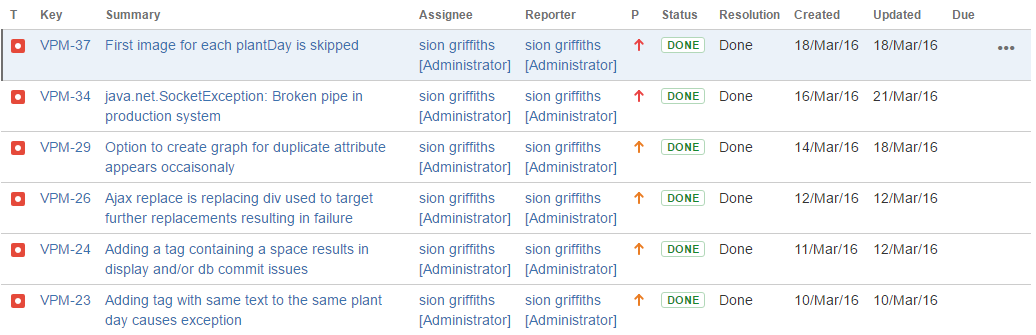
\includegraphics[width=\textwidth]{images/tools/jira_bugs}
    \caption{A sample of bugs raised in Jira}
    \label{fig:jira_bugs}
\end{figure} 

Another helpful feature was the integration with the version control repository hosted on Github. Referencing the issue ID in Jira in a commit message linked the commits with the issue within Jira. This provided a handy way to track development against particular issues over time and allowed a quick way to navigate between the issues in Jira and the commits on Github. 

\begin{figure}[H]
    \centering
    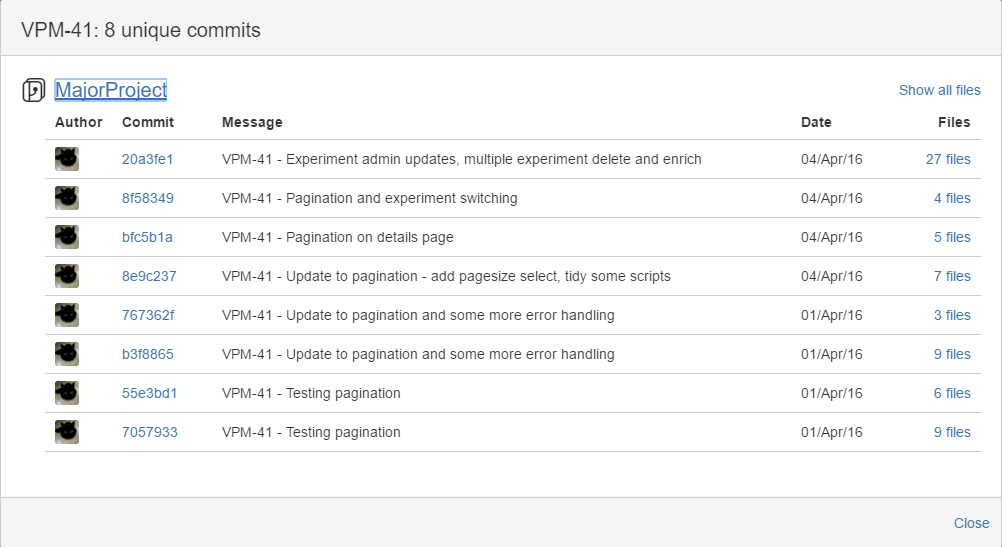
\includegraphics[width=\textwidth]{images/tools/jira_commit}
    \caption{The version control commit tracking within Jira}
    \label{fig:jira_commit}
\end{figure} 

There are a vast array of alternatives that could have been used for issue tracking within the project, many provide the full array of features that were used in Jira during the development of this project. However, Jira being the industry leader, provided an opportunity to gain further valuable experience of its use in a day to day, agile development project. Having previously been involved in the running of a Jira system during my time in industry provided me with familiarisation in configuring a project for my needs and confidence in being able to do so quickly. This was enough to chose Jira over the alternatives that were evaluated such as Waffle.io and the native issue tracking feature provided with Github.

\subsection{Codeship} 
Codeship\cite{_codeship} is a web based Continuous Integration(CI) service. Working in conjunction with the version control repository, Codeship will detect up any commits made to the repository hosted on Github and execute build and test scripts defined as part of the initial setup of the CI service. Use of a CI system within the project provided assurance that each incremental change made to the system integrated correctly and that all tests continued to pass. A notification would be sent in the event of build or test failure.  

 The build script for the project can be seen in figure~\ref{fig:build_script} showing how the project databases are setup and the environment is configured prior to executing the project build and test commands.

 The scripts are invoked within small Docker \cite{docker} based environments which allow build dependencies to be modularised and configured quickly. The initial integration of the CI system into the project environment was extremely simple, linking the Github repository for the project was a couple of mouse clicks and the script below is the entirety of the extra configuration required to get the CI system fully up and running. It was because of this speed and simplicity of configuration that Codeship was chosen over rival offerings such as TravisCI \cite{travis} which appeared to have a much more complex initial setup during evaluation.

\begin{figure}[H]
    \centering
    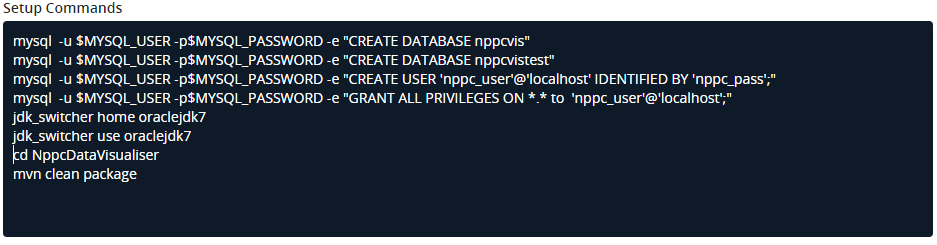
\includegraphics[width=\textwidth]{images/tools/codeShipScript}
    \caption{The project build script on Codeship}
    \label{fig:build_script}
\end{figure} 

\begin{figure}[H]
    \centering
    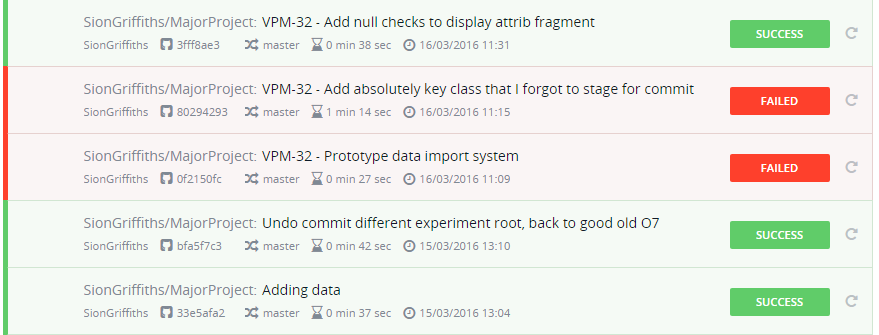
\includegraphics[width=\textwidth]{images/tools/codeShipSmall}
    \caption{A sample of the build history in Codeship}
    \label{fig:build_history}
\end{figure} 



\subsection{Plotly.js}

Plotly.js\cite{_plotly} is an open source graphing library built on top of technologies such as d3.js, a Javascript data manipulation and visualisation library, and stack.gl, a wrapper around WebGL and other associated technologies. There are numerous alternatives libraries that could have been chosen, including d3.js itself and Google Charts amongst others, but the ease of integration with the system and the look and feel of the output from Plotly.js made it the superior choice for this project. Figure~\ref{fig:plotly} shows a Plotly.js generated graph embedded within the Graphs page in the system.


\begin{figure}[H]
    \centering
    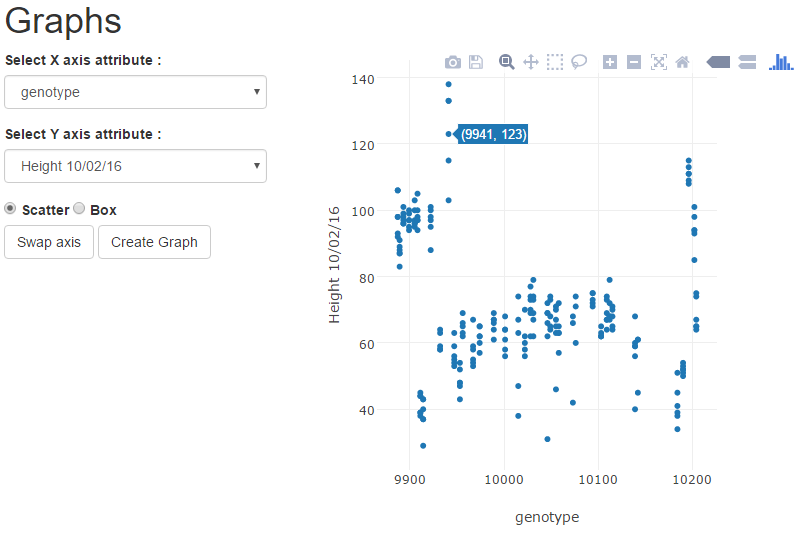
\includegraphics[width=\textwidth]{images/design/plotly}
    \caption{Project graph page featuring a Plotly.js generated graph}
    \label{fig:plotly}
\end{figure} 

\chapter{Implementation}



\section{Integration with NPPC data repository}
Fairly straight forward, recursive methods slow, iterative and tightly coupled fast
The structure of the data repository changed soon after implementation was begun
\section{Graphing System}
Wrapping things into nice JSON format for plotly, fun with join queries.

\section{Domain model implementation and ORM}
Talk about looping references and stack overflows? Laze/eager fetch? 

\section{Data Import}
Use of the arrays to hold column values "hashing" the values into the right place using the numbers in the list

\section{IBERS hosted environment}

\chapter{Testing}

\section{Overall Approach to Testing}

The overall approach to testing was to have high test coverage of system features and functionality and to automate these tests wherever it was feasible to do so. Automated tests would run often as part of the normal development workflow and provide continuous assurance of functionality and system environments. Where automation was impractical, alternative approaches were taken to ensure that the system was fully tested in a robust manner.

\section{Automated Testing}

For the purposes of automated testing, a separate database was used. The database would be completely recreated for the start of each run of the test suite and dropped at the end. Prior to the tests running, the database would be seeded with test data that is similar to the real world data expected in the production database. By using this method the tests would more closely mirror the real world behaviours of the system and each run could be insulated from the data changes made in previous runs.

A Continuous Integration(CI) system was used in order to facilitate the convenient and regular running of all automated tests in the project. The CI system would build the project from source each time a commit was made into the version control repository. As part of this build process the full test suite would be run. Any issues encountered during this process, from compilation errors to test failures, would result in the build being rejected by the CI system. In the event of a rejected build, the CI system would notify via email of the build failure. This feature turned out to be invaluable since it highlighted a configuration issue that did not affect my local development environment but would have affected the server the project is hosted on. Because the tests were automated and I was notified of a failure, I saved what likely would have been a significant amount of debugging time at the next release of the project to the server. Time was also saved since the full test suite didn't need to be run locally at development time, single tests could be run and the full test and integration suite would be invoked on commit to the version control repository. 

Figure \ref{fig:testrel} shows the test results page for the automated tests as generated by Intellij when the full test suite is executed locally. Certain tabs within the page are expanded for display purposes.

\begin{figure}[H]
    \centering
    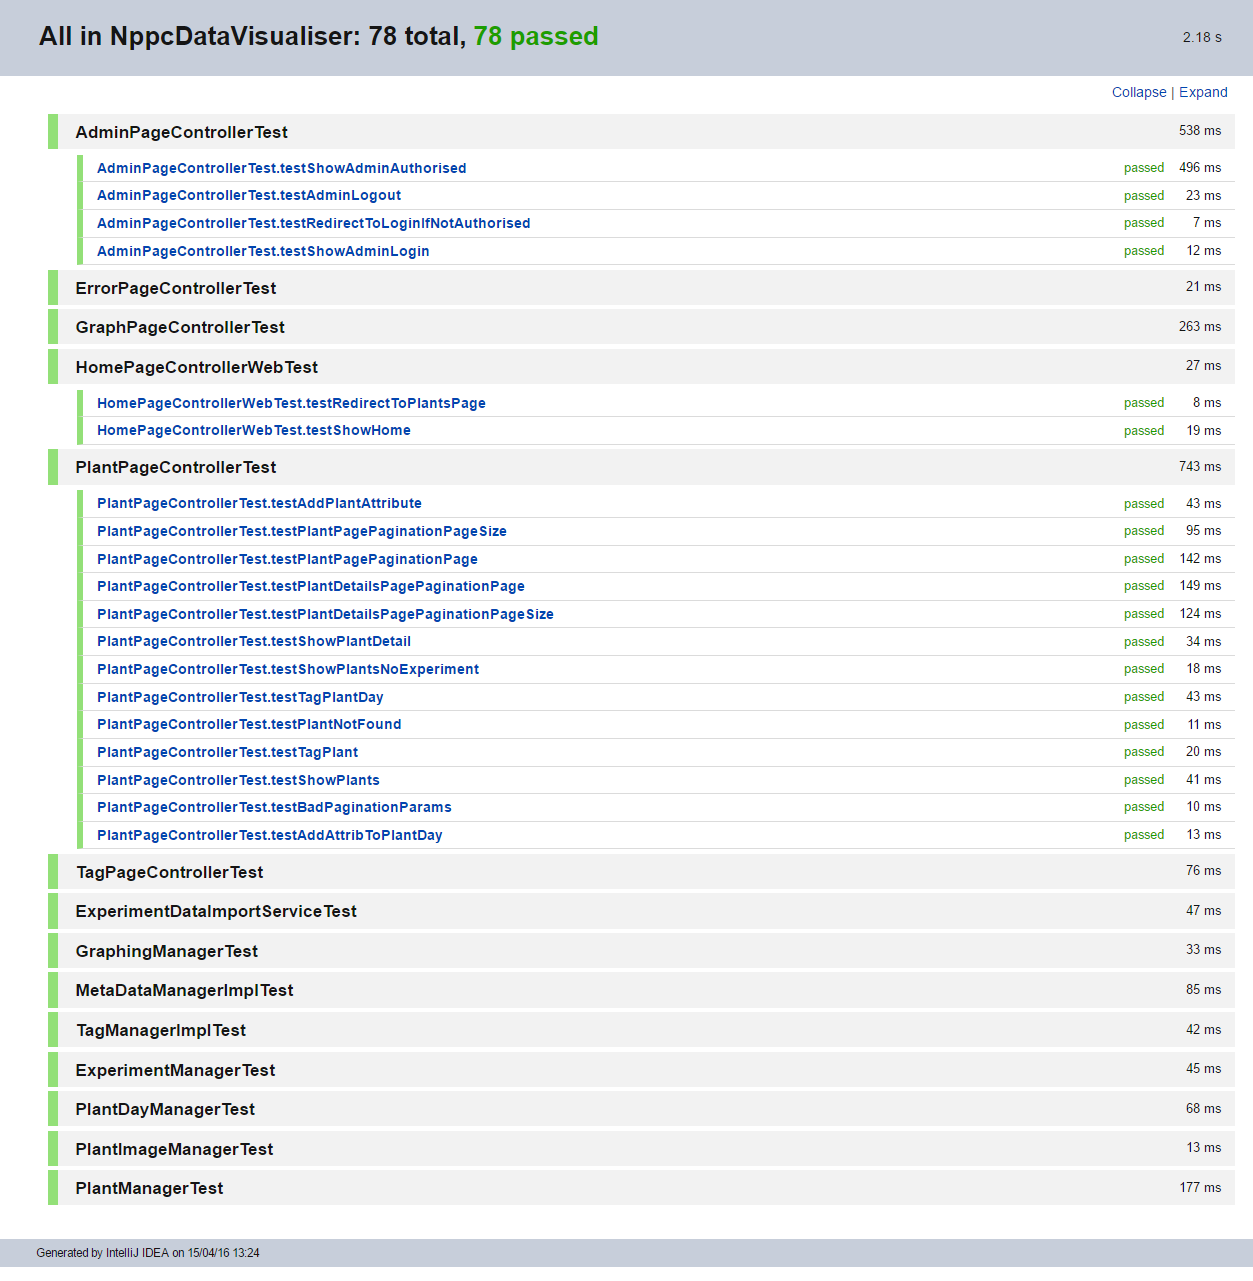
\includegraphics[width=\textwidth]{images/testing/results}
    \caption{Automated test result page generated by Intellij }
    \label{fig:testrel}
\end{figure} 

\subsection{Unit Tests}

 When implementing most of the service layer classes for the system a TDD approach was employed in order to ensure high test coverage of the parts of the system which incorporate the business logic. Using TTD helped evolve the design of these service classes by ensuring that nothing was built in a way that was difficult or convoluted to test. Tests are implemented on a method by method basis for the most part, that is, each method in a service will have its own unit test to ensure functionality.
 
  A simple example is shown in listing~\ref{lst:jUnit} detailing a test for the tags reset functionality in the PlantManager service class that is invoked as part of deleting the data associated with an experiment.
\lstjava
\lstinputlisting[label={lst:jUnit},caption=Unit test for the PlantManager service]{sourceCode/mySnippets/testing/testResetTags.java}
Most of the classes not covered by unit testing are tested via integration testing. The overall coverage for automated tests in the system is 79 \% of all lines written in Java.

\subsection{Integration Testing}

Integration testing for this project was achieved primarily through testing of the MVC controller classes. The goal behind these tests was to make requests to the various available routes within the system and verify that the correct results are returned. Being a web based system, all functionality is in some way linked to a request mapping or route in a controller class. Testing these routes provides a convenient method to ensure the distinct layers and components that make up the system are working as intended and the interactions between them are as expected. 

Integration tests for this project take advantage of features provided by the Spring framework in order to simplify the configuration of the tests and the mocking of certain aspects of the system, such as the application context in which the tests are running. These mocked dependencies and use of the same static data and database each run ensure that results can be verified consistently.

 The example test in listing~\ref{lst:integrationTest} shows how a mockMvc object is used to simulate the web application context and perform requests against the application, in this case a HTTP GET to the path `/plants' which should return the plants page. The HTTP session object can be managed as part of the tests and injected into individual requests to ensure compatibility with real world usage. Following the HTTP request the results can be verified, in the case of the example test the HTTP status is checked to ensure that the server returned status code 200 (Ok). The content of the response is verified then finally, a check against the view() method is made to ensure that the correct page has been returned as a result of the request. 

\lstinputlisting[label={lst:integrationTest},caption=Simple integration test example]{sourceCode/mySnippets/testing/testShowPlants.java}

A similar approach is adopted for all integration tests throughout the system. For each tested route, the request is simulated and results verified in much the same way as in the example test. In more complex tests or those testing functionality which require more robust verification there are extra steps taken such as asserting the existence of certain page model attributes or objects being passed to the front end views.


\subsection{Stress and Performance Testing}

Performance and stress testing was carried out through the use of Apache Jmeter\cite{_jmeter}, an open source Java application built to measure site and application performance under controlled loads. Jmeter enables the simulation of a number of concurrent users accessing a given site, these simulated agents follow a defined sequence of actions as specified in the test script. Unless otherwise stated the tests run with ten concurrent agents and the tests are repeated thirty times in order to smooth out any outliers in the data.

The tests were all carried out against the project hosted on the remote server provided by Ibers. The machine used to run the Jmeter scripts is a powerful desktop machine using a recent generation of Intel i7 processor featuring 4 cores and able to process 8 concurrent threads. It is necessary that the test machine be connected to the Aberystwyth University VPN in order to reach the target server although the impact of the extra overhead appears minimal and is considered for the sake of comparing results. Although the ten concurrent users may seem low, the throughput on average is over 100 requests per second when run from the test machine which is significantly more than ten real users would be able to generate.

For the purposes of this project Jmeter was used to assess whether pages in the site would load within defined time limits and whether implementation decisions have an adverse effect on performance. In general the goal was to have pages served within 300ms with a hard limit of 1000ms, or one second, although this does not include image load times. A target of 300ms is well under the 1 second limit for keeping a users flow of though as identified as part of a study conducted by Nielsen \cite{responseTimes}. Running the tests regularly could also help highlight issues that may not be uncovered under other forms of testing such as intermittent problems that could result in request errors that would be difficult to reproduce otherwise.


General results as output by Jmeter are included in figure~\ref{fig:jmeter_with_data} for an experiment which has been initialised with data. The initialisation is an important distinction because the amount of experiment data significantly affects the initial page response time for the Graphs page, other pages are affected somewhat but to a much lesser degree. Figure~\ref{fig:jmeter_no_data} displays the results of running the same test without the data having been added to the experiment and it's clear to see the effect on the load time for the Graphs page. Having these results available during development informed some of the design choices within the Graph page such as having the graphs themselves and any plant objects loaded via Ajax following user interaction as opposed to being populated into the page on load.
\begin{figure}[H]
    \centering
    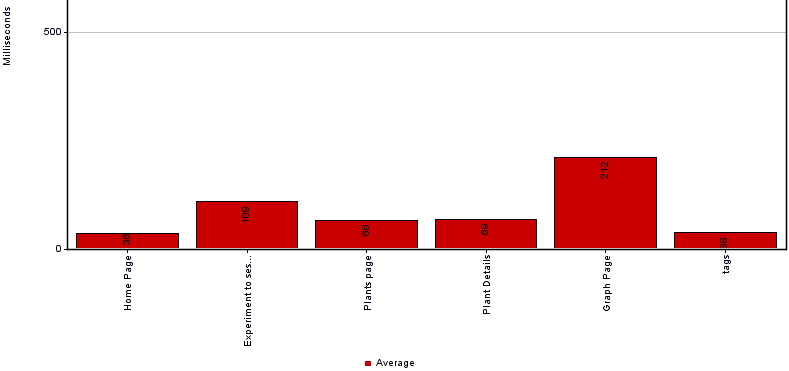
\includegraphics[width=\textwidth]{images/testing/jmeter_final_crop}
    \caption{Visulisation of Jmeter test result of a fully initialised experiment}
    \label{fig:jmeter_with_data}
\end{figure} 

\begin{figure}[H]
    \centering
    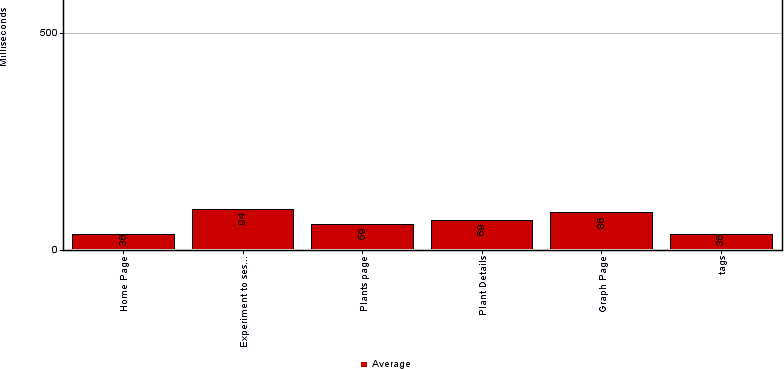
\includegraphics[width=\textwidth]{images/testing/jmeter_no_data_crop}
    \caption{Visulisation of Jmeter test result of a partially initialised experiment}
    \label{fig:jmeter_no_data}
\end{figure} 

The effect of choosing pagination defaults for the plants and plant detail pages could also be measured although in the case of pagination the real limiting factor is the bandwidth and render time required. However, the effect on request time and loading on the server could be seen and monitored for any potential issues. In an experiment with many plants or a large amount of data the response time would increase significantly with page sizes of over 50 or so plants but no other adverse affects were noticed on the system even with a significant number of requests.



\section{Manual Testing}
For areas of the system where automated testing was impractical or insufficient to verify results, a manual approach was taken and test tables used to verify functionality is as expected. 

\subsection{Admin Page Test Table}
Much of the functionality on the Admin page relies on an active network connection to the NPPC data repository and as such is unsuitable for automated testing. There was no feasible way to establish a connection between the continous integration server and the NPPC data repository therefore the manual verification of functionality is necessary.
\begin{table}[H]
\centering
\begin{tabular}{ | p{4cm} | p{4cm} |p{4cm} | p{1cm} | }
\hline
	\textbf{Test} & \textbf{Input} & \textbf{Expected Output} & \textbf{Pass} \\ \hline
	Attempt to access admin area without login & Go to /admin without login & Redirected to administrator login page & \checkmark \\ \hline
	Attempt to access admin area with correct login & Go to /admin with login & Admin is page is displayed & \checkmark \\ \hline
	Attempt admin login with incorrect credentials & Submit admin login form with incorrect credentials & Error displayed to user. & \checkmark \\ \hline
	Admin log out & Click logout button from admin page & Redirect to home page and authorisation cleared from session & \checkmark \\ \hline
	Initialise Experiment & Click initialise button for uninitialised experiment & Experiment begins initialising - plants are created & \checkmark \\ \hline
	Update experiment & Click Update button on initialised experiment & Experiment begins update, plants are updated or created & \checkmark \\ \hline
	Import data with valid csv & Click Init Data button on initialised experiment & Data is imported from csv & \checkmark \\ \hline
	Import data with invalid csv & Click Init Data button on initialised experiment & Invalid csv data is ignored & \checkmark \\ \hline
	Delete data & Click delete data on experiment & Data is deleted from the experiment & \checkmark \\ \hline
	Delete plants & Click delete plants button on experiment & Plant data and images are deleted & \checkmark \\ \hline
\end{tabular}
\caption{Test Table for Admin page functionality}
\label{test_table_admin}
\end{table}
\subsection{Graph Page Test Table}
Although most of the functionality within the Graph page is verified via automated testing, certain aspects require visual verification and as such a manual approach is taken to verify functionality within the page.
\begin{table}[H]
\centering
\begin{tabular}{ | p{4cm} | p{4cm} |p{4cm} | p{1cm} | }
\hline
	Test & Input & Expected Output & Pass \\ \hline
	Test view graphs with no experiment & Go to /graphs with no selected experiment & No data' page is show with back button & \checkmark \\ \hline
	Test view graphs with experiment that has no  data & Go to /graphs with experiment in session that has no data & No data' page is show with back button & \checkmark \\ \hline
	Test view graphs with experiment that has data & Go to /graphs with experiment in session that has data & Graph page is shown with graph creation options & \checkmark \\ \hline
	Test create graph & Click create graph button on /graphs page & A graph is displayed in the page with selected axis attributes & \checkmark \\ \hline
	Test box plot & Select 'Box' and create graph & Nodes in the graph are represented as box plots & \checkmark \\ \hline
	Test scatter plot & Select 'Scatter' and create graph & Nodes in the graph are represented as scatter plot & \checkmark \\ \hline
	Test swap axis & Click swap axis button & Selected axis attributes are swapped, x value becomes y value and vice versa & \checkmark \\ \hline
	Test plant results on graph node click & Click on or near a node in the graph & A  clickable list of plants corresponding to the values of the clicked node appear in the page & \checkmark \\ \hline
	Test click result plant & Click on a plant link generated as result of clicking on a graph node & User is redirected to the detail page for the clicked plant link & \checkmark \\ \hline
\end{tabular}
\caption{Test Table for Graph page functionality}
\label{test_table_graph}
\end{table}


\section{User Testing}

When development was near complete a small sample of volunteer test users were recruited to use the system and give feedback on usability and the system in general. An online form was provided with a number of questions and a section for general feedback the responses to which can be found in Appendix %!TODO sort appendix linking

Following the user testing, a number of changes were implemented according to the feedback given. Namely, adding pagination controls to the bottom of the plants and plant detail pages for more convenient page navigation and fixing an overlooked issue on the plant detail graph page. If a plant has no attributes recorded against individual plant days then the page should make the user aware that graph generation is not possible and provide a means to return to the previous page. Prior to user testing the page was confusing and mostly blank in the event that no graphable data was available.



\chapter{Evaluation}

Examiners expect to find in your dissertation a section addressing such questions as:

%\begin{itemize}
%   \item Were the requirements correctly identified? 
%   \item Were the design decisions correct?
%   \item Could a more suitable set of tools have been chosen?
 %  \item How well did the software meet the needs of those who were expecting to use it?
%   \item How well were any other project aims achieved?
%   \item If you were starting again, what would you do differently?
%\end{itemize}

%Such material is regarded as an important part of the dissertation; it should demonstrate that you are capable not only of carrying out a piece of work but also of thinking critically about how you did it and how you might have done it better. This is seen as an important part of an honours degree. 

%There will be good things and room for improvement with any project. As you write this section, identify and discuss the parts of the work that went well and also consider ways in which the work could be improved. 

%Review the discussion on the Evaluation section from the lectures. A recording is available on Blackboard. 


\section{Requirements}




\section{Implemented System}
\subsection{Strengths}
\subsection{Weaknesses}
\subsection{Future Work and Improvements}

The project brief was fairly open ended and the delivered system fairly narrow in scope, this leaves many avenues for potential improvement and expansion of the system, potential examples of which are discussed  below :

\subsubsection{Search and filtering}
Further utility could be provided by the system if some extensive search and filtering functionality was implemented. Filtering the time series of images or plants in an experiment by attribute values, ranges etc would enhance the ability of the user to find specific information of interest or aid in inputting such specific data to particular entities within the system. Similarly, searching for plants or attribute values would be a helpful utility in both exploration of the experiment data and input of data to specific entities of interest within the system.

One approach which was partially investigated during the implementation was to use the Elasticsearch\cite{elastic} integration provided by Spring. This implementation provides a means to index certain attributes and classes within the system to provide a convenient and fast solution to searching and filtering. The approach follows a similar principle to that implemented for the persistence layer, that is, the entity classes are annotated and a `data repository' interface is used to query these entities, further details can be found in the Spring documentation\cite{_spelastic}  


\subsubsection{Comparisons and statistical analysis}
As the interesting results of experiments carried out at the NPPC are often statistical in nature it would be convenient to the scientists using the system to be able to conduct or view the results of simple statistical analysis alongside the visualisation of data provided by the delivered system. As discussed in previous sections, the scientists conducting experiments often analyse only very narrow ranges of data correlations that could be present in an experiment. Providing a correlation measure for graphed attributes could indicate to users of the system that interesting correlations exist in previously overlooked data. 

When generating a graph visualisation from two attributes, a correlation measurement could be taken between the two attributes using the entire set of examples within the experiment. One such method would be to use Spearmans rank correlation coefficient\cite{spearman} to display the correlations between attributes. There are various libraries available within the Java ecosystem that provide implementations of such statistical analysis algorithms and methods. 

\subsubsection{Machine learning}
With the potential for large datasets of meaningful, well understood data that is often statistical in nature it is an ideal scenario to leverage some machine learning capability in order to produce potentially interesting correlations and conclusions from system data. The main obstacle to providing such a facility is the current lack of collected data within the context of experiments. If the system was used mroe extensively then the provision of machine learning would become more and more feasible. Data for ongoing experiments recorded within the system could be used to provide the basis of predictions of certain traits and attributes which could, if sufficiently accurate, provide the scientists with the means to focus effort on the most interesting, promising or relevant subset of plants within an experiment.



\subsubsection{Image processing and computer vision}
The NPPC captures vast quantities of image data for each experiment. Different modalities and angles add to the richness of the images as a potential data source in themselves. There is a wide array of potential improvements to the system that could be made to take advantage of such data. The NPPC themselves are concerned with the leverage of computer vision approaches to image analysis with ongoing research into useful automated procedures such as the detection of specific growth stages in oats as developed by Boyle et al\cite{boyle_image-based_2015}. As a result there are automated processes that provide support to the deployment of image based processes such as segmentation of images to provide masks of plant pixel location within images.

The system could be extended to use popular image processing libraries such as ImageJ (integration of which was tested briefly during spikework and verified as viable) which can provide many useful functions such as pixel colour maps, counts and so forth which could be used to infer the health or age of a given plant, detect fungus and so on. 

It is possible to invoke external programs using system calls from within the delivered system, it is not infeasible to run compatible experiments through detectors such as that developed by Boyle et al\cite{boyle_image-based_2015} in order to automate the detection of certain growth stages and record these results within the persistence layer of the system


\subsubsection{Comprehensive user management}
Within the delivered system there is only the concept of an admin user and generic users. Providing the means for users to register and create account opens up many interesting options for further development of the system. In providing individual user accounts it is possible to then extend the attribute system to allow a concept of ownership, for example if a user adds attributes to a plant then that user has ownership of that attribute and gains the ability to delete or edit the attribute. Other users could raise disputes against the attribute or provide a competing value for the same attribute, this would allow the system to score agreement on particular assessments of certain traits or characteristics as identified by the different stakeholders within an experiment. Providing an agreement score for attributes in such a manner would provide a more robust dataset for use in other applications such as machine learning or vision systems.

A popular approach to encouraging user participation within such systems is gamification (bringing elements of game-design into non-game contexts), a system where users can gain points or extended privileges based on participation could be used to encourage scientists to add data and utilise the system more fully. 




\section{Process}

It is believed that an agile approach as chosen for this project was the correct choice and that the process followed during the course of this project was successful for a number of reasons. It provided an environment in which work could be effectively prioritised based on emergent or short term needs and goals without having to reorganise more than the current day or iterations work. Being able to react to change and bugs in this way made development more comfortable especially when requirements were not concrete and the domain was not fully understood at the beginning of iterations. Other approaches may not offer such a degree of flexibility.

The use of user stories and the ability to move them into and out of the scope of iterations along with progressing their status made the project work flow more easily and allowed the focus to be on the goal of an iteration and the next release rather than a generic list of un-organised tasks.  As discussed in Section~\ref{proc}, the estimation of tasks in terms of time could have been improved to provide a more complete understanding of developer throughput which would have led to more efficient allocation of pomodoros to the correct tasks. However, estimation is notoriously difficult to do with a high degree of accuracy especially when working with technologies that developers aren't fully experienced in using.

A key part of the process followed is the incremental and frequent release of the product. Providing a deployment at the end of each iteration offered a source of reassurance to stakeholders that work was progressing and also provided, via the use of version control facilities, the opportunity to rollback if a release was broken or problematic.

\section{Student Evaluation}
%\subsection{General}
There are a number of areas which could have been improved when considering personal performance during the course of this project. Most notably a more proactive approach to engaging with the plant scientists at the NPPC would have brought benefits to the project in terms of delivering a more useful system and focusing on providing functionality that would improve their interactions with the system. A tenuous offer of co-location was made such that a hot desk could have been available at the NPPC for the duration of project work which would have allowed a closer working relationship with the staff at the NPPC. In taking these more proactive approaches, more time could have been freed to implement some of the more interesting improvements discussed in the previous section, this is the source of a little regret and results in a changed attitude towards how work is approached in general.

The approach to time management was greatly improved as a result of this project, when it seemed that much time was being wasted in unfocused effort, this was rectified by implementation of, and dedication to, the pomodoro technique resulting in more productive output in fewer hours then before the adoption of the technique.

The project provided the opportunity to learn about an interesting domain that otherwise would not have been available and to meet with inspiring people who enjoy their field of work.
%\subsection{Take homes}
% add any additional chapters here

\setemptyheader
\addcontentsline{toc}{chapter}{Appendices}
\chapter*{Appendices}
\pagebreak

% start the appendix - sets up different numbering
\fancypagestyle{plain}{%
%\fancyhf{} % clear all header and footer fields
\fancyhead[L]{\textsl{Appendix\ \thechapter}}
\fancyhead[R]{\textsl{\leftmark}}}

\appendix
\fancyhead[L]{\textsl{Appendix\ \thechapter}}
\fancyhead[R]{\textsl{\leftmark}}
\fancyhead[C]{}
\fancyfoot[C]{\thepage}
\renewcommand{\headrulewidth}{0.4pt}
\renewcommand{\chaptermark}[1]{\markboth{#1}{}}

\fancyhead[L]{\textsl{Appendix\ \thechapter}}
\fancyhead[R]{\textsl{\leftmark}}
\fancyfoot[C]{{\thepage} of \pageref{LastPage}}

% include any appendices here
\chapter{Third-Party Code and Libraries}

plotly
jquery
bootstrap
spring?

\chapter{Ethics Submission}

%This appendix includes a copy of the ethics submission for the project. After you have completed your Ethics submission, you will receive a PDF with a summary of the comments. That document should be embedded in this report, either as images, an embedded PDF or as copied text. The content should also include the Ethics Application Number that you receive. 



\includepdf[pages={1,2}, scale = 0.7]{pdfs/ethics.pdf}
\chapter{Code Examples}

\section{Random Number Generator}

The Bayes Durham Shuffle ensures that the psuedo random numbers used in the simulation are further shuffled, ensuring minimal correlation between subsequent random outputs \cite{NumericalRecipes}.

\begin{verbatim}
 #define IM1 2147483563
 #define IM2 2147483399
 #define AM (1.0/IM1)
 #define IMM1 (IM1-1)
 #define IA1 40014
 #define IA2 40692 
 #define IQ1 53668
 #define IQ2 52774
 #define IR1 12211
 #define IR2 3791
 #define NTAB 32
 #define NDIV (1+IMM1/NTAB)
 #define EPS 1.2e-7
 #define RNMX (1.0 - EPS)
 
 double ran2(long *idum)
 {
   /*---------------------------------------------------*/
   /* Minimum Standard Random Number Generator          */
   /* Taken from Numerical recipies in C                */
   /* Based on Park and Miller with Bays Durham Shuffle */
   /* Coupled Schrage methods for extra periodicity     */
   /* Always call with negative number to initialise    */
   /*---------------------------------------------------*/	
 
   int j;
   long k;
   static long idum2=123456789;
   static long iy=0;
   static long iv[NTAB];
   double temp;
 
   if (*idum <=0)
   {
     if (-(*idum) < 1)
     {
       *idum = 1;
     }else
     {
       *idum = -(*idum);
     }
     idum2=(*idum);
     for (j=NTAB+7;j>=0;j--)
     {
       k = (*idum)/IQ1;
       *idum = IA1 *(*idum-k*IQ1) - IR1*k;
       if (*idum < 0)
       {
         *idum += IM1;
       }
       if (j < NTAB)
       {
         iv[j] = *idum;
       }
     }
     iy = iv[0];	
   }
   k = (*idum)/IQ1;
   *idum = IA1*(*idum-k*IQ1) - IR1*k;
   if (*idum < 0)
   {
     *idum += IM1;
   }
   k = (idum2)/IQ2;
   idum2 = IA2*(idum2-k*IQ2) - IR2*k;
   if (idum2 < 0)
   {
     idum2 += IM2;
   }
   j = iy/NDIV;
   iy=iv[j] - idum2;
   iv[j] = *idum;
   if (iy < 1)
   {
     iy += IMM1;
   }
   if ((temp=AM*iy) > RNMX)
   {
     return RNMX;
   }else
   {
     return temp;	
   }
 }
 
\end{verbatim}



\fancypagestyle{plain}{%
   \fancyhead{} %[C]{Annotated Bibliography}
   \fancyfoot[C]{{\thepage} of \pageref{LastPage}} % except the center
   \renewcommand{\headrulewidth}{0pt}
   \renewcommand{\footrulewidth}{0pt}
}

\setemptyheader

\nocite{*} % include everything from the bibliography, irrespective of whether it has been referenced.

% the following line is included so that the bibliography is also shown in the table of contents. There is the possibility that this is added to the previous page for the bibliography. To address this, a newline is added so that it appears on the first page for the bibliography. 
\addcontentsline{toc}{chapter}{Annotated Bibliography} % Adds References to contents page

%
% example of including an annotated bibliography. The current style is an author date one. If you want to change, comment out the line and uncomment the subsequent line. You should also modify the packages included at the top (see the notes earlier in the file) and then trash your aux files and re-run. 
%\bibliographystyle{authordate2annot}
\bibliographystyle{IEEEannot}
\renewcommand{\bibname}{Annotated Bibliography} 
\bibliography{References/zotero} % References file


\end{document}
